\documentclass{scspaperproc}

\usepackage{latexsym}
\usepackage{graphicx}
\usepackage{mathptmx}
\usepackage{ulem}

% To do: here's how Stephen compiles the paper from the ANNSIM directory:
% pdflatex scs23paper.tex 
% bibtex scs23paper
% pdflatex scs23paper.tex
% pdflatex scs23paper.tex
%
% By putting this into an alias in my .bashrc with:
% alias lt="pdflatex scs23paper.tex ; bibtex scs23paper ; pdflatex % scs23paper.tex ; pdflatex scs23paper.tex"
% I can compile the paper to a PDF in one shot.
%
% When adding new papers to Zotero, be sure to put them in the ANNSIM folder
% (or subfolder), then highlight all and Export... to BibTex mode, saving the
% file under the name bib.bib (in assets subdirectory). Don't forget to commit
% your changes to bib.bib as well as your changes to any of the .text files!


\usepackage[pdftex,colorlinks=true,urlcolor=blue,citecolor=black,anchorcolor=black,linkcolor=black,bookmarks=false]{hyperref}

% Avoid overrunning the right margin; you are welcome to remove this, provided that you take care not to overrun the right margin anywhere in your paper
\sloppy

\begin{document}

\SCSpagesetup{Davies and Peura}

\def\SCSconferencename{Annual Simulation Conference}

\def\SCSconferenceacro{ANNSIM'24}

\def\SCSpublicationyear{2024}

\def\SCSconferenceeditors{P.J. Giabbanelli, I. David, C. Ruiz-Martin, B. Oakes and R. C\'{a}rdenas}

\def\SCSconferencedates{May 20-23}

\def\SCSconferencevenue{American University, DC, USA}

\title{THE INTERACTION BETWEEN HETEROGENEOUS VOTING STRATEGIES AND DYNAMIC
VOTE-SEEKING CAMPAIGNS: AN AGENT-BASED MODEL}

\textit{(Author names/affiliations to be redacted for initial blind submission.)}
\author[\authorrefmark{1}]{\sout{Stephen Davies}}
\author[\authorrefmark{1}]{\sout{Harmony Peura}}

\affil[\authorrefmark{1}]{\sout{University of Mary Washington Computer Science,
Virginia USA}}
\affil[ ]{\textit {\sout{stephen@umw.edu}}}
\affil[ ]{\textit {\sout{hpeura@umw.edu}}}


\maketitle

\section*{Abstract}

Political candidates in a democracy articulate positions on the issues of the
day, but they are also highly aware of voter sentiment on those issues, and
tailor their campaigns accordingly as they seek to win elections. Voters, too,
adjust their political opinions based on (among other things) interactions with
others in their social network. We present an agent-based simulation that
models this dynamic interplay between candidates and voters, in order to shed
light on what outcomes candidates can expect to result from a policy of
``chasing'' votes. The voters in our simulation differ from one another in the
decision procedure they use in choosing who to vote for -- these voting
algorithms are modeled on results from the political science literature about
the different ways voters make decisions. Our model can thus be used to
experiment with a virtual electorate, to determine the conditions under which
vote-chasing candidates gain an advantage or perhaps even cause the election
outcome to be objectively irrational.


\textbf{Keywords:} opinion dynamics, ABM, election, voting

\section{Introduction}
\label{sec:intro}

Many factors are known to influence voters in democratic elections, including
their own background characteristics (demographics, ideology, partisanship,
personality traits, \textit{etc.}), the distinctiveness of the candidates, the
availability of information, and the voter's perception of their
identity.\cite[pp.3-4]{redlawsk_citizens_2020} But another major factor -- and
one we would argue \textit{should} be the most important, if citizens are
casting their votes rationally -- is the candidates' stance on the issues of
the day. At least in principle, voters are electing the candidate who will
enact policies most favorable to them if elected to office.



\section{Related work}
\label{sec:related}

% Key aspects of SD/HP: graph, opinion space, elections, modeling (not
% forecasting)

% No opinion space
In many approaches to modeling elections, voters' attitudes towards the parties
comprises merely a valence and possibly a magnitude, rather than involving a
more complex amalgamation of issue positions. The original binary voter model,
for example, utilized only a single ``issue'' upon which an individual could
hold a position.\cite{holley_ergodic_1975,clifford_model_1973}. Even in
Kottonau and Paul-Wohstl's much more recent seminal
work\cite{kottonau_simulating_2004}, citizens maintain a ``mental accounting''
of only a single variable over the course of an election season -- namely,
which of the two parties they favor. The campaigns for these parties then
attempt to optimize their advertising resources to influence would-be voters at
opportune times. Burke and Searle\cite{burke_quantitatively_2022} followed
Sobkowicz's emotion/information/opinion (E/I/O)
approach\cite{sobkowicz_quantitative_2016} in making agents' mental states more
complex and realistic: in addition to holding a certain opinion about a party
(or candidate), an agent is, at any moment, in either a ``calm'' or
``agitated'' state, which controls how they influence and are influenced by
other agents (and by campaign messaging). Here, too, the object of analysis is
a single ``issue'' (pro party A or B), not an array of them.

Our model, in contrast to all of these, the main levers available to a campaign
are the party's issue positions, which they can adjust in an attempt to woo
voters.


% Opinion space done differently

% Jung et al 2021
%   multiple issues, but opinions on each one is binary
%   adjacent-numbered issues are presumed to be semantically related to each
%     other. an agent having all 0's, or all 1's, is interpreted as being
%     "consistent" in some way.
%   the main influencing dynamic is not pairwise, but *groupwise*. (considering
%     an agent's entire ingroup.)

% Sîrbu et al 2013  "vector of values, but not in the same way as ours;
%   instead, the vector represents multiple possible positions on a single
%   issue (e.g., agent A is .3 "permanent cease fire in Gaza", .2 "temporary
%   cease fire in Gaza," .5 "increase US funding to Israel in fighting
%   Hamas.")"




% Election forecasting
Recently, Gao \textit{et al}\cite{gao_forecasting_2022} have presented a
promising approach to election forecasting. They combine current demographic
attributes of the population with historical results of past election outcomes
in order to determine how much each attribute is likely to influence voters,
and in which direction. This is very different from our model, both in purpose
(actually forecasting upcoming elections, rather than exploring ``what if?''
voting strategy scenarios) and in approach (the agents in
\cite{gao_forecasting_2022} do not influence one another on a social network.)

The emotion/information/opinion (E/I/O) approach, utilized by both
\cite{sobkowicz_quantitative_2016} and, more recently,
\cite{burke_quantitatively_2022}, can lead to less rigidity in model outcomes
and perhaps even conditions conducive to legitimate third parties coming into
play.

% Harmony's unorganized notes
Laver:
\begin{itemize}
\item looks at the continuous dynamics of political competition with no regard for elections
\item analyzes different strategies party leaders can continuously employ to get support from voters- they treat this as an IV, we treat it as a DV
\item deployed model in a way to retrieve a real opinion poll series in Ireland
\end{itemize}
Lehrer et al:
\begin{itemize}
\item extension of Laver's model: parties form coalition governments and parties have utility functions (they are motivated by more than just votes)
\item they look at how different party adaption strategies can lead to opitmal representation in both parties and the government, whereas we look at how different voting algorithms lead to different vote distributions
\item they hold elections, but all voters vote rationally whereas we explore different voting algorithms
\end{itemize}
Wright and Sengupta:
\begin{itemize}
\item extension of Laver's model: uses their "hunter" campaigning  strategy
\item analyzes the impact of lobbying oligarchs on the political system
\item no elections or voting, they only look at party dynamics
\end{itemize}

\section{The model}
\label{sec:model}

\subsection{Overview}

An abstract \textbf{opinion space} is represented as a continuous
$I_N$-dimensional Euclidean space, where $I_N$ is the number of issues. An
\textbf{opinion} $O_i$ on \textbf{issue} $I_i$ is a value in the real interval
$[0,1]$, for $1 \leq i \leq I_N$.

There are two kinds of agents in the model: $C_N$ \textbf{candidates}, and
$V_N$ \textbf{voters}. Agents of either type each have a dynamic
\textbf{opinion vector} $(O_{i_1}, O_{i_2}, O_{i_3}, ..., O_{i_{I_N}})$
comprising one opinion on each issue; in other words, a point in the opinion
space.

A random Erd\H{o}s-R\'{e}enyi graph\cite{erdhos_evolution_1960} is generated
with $V_N$ nodes and uniform edge probability of $p_e$. During each iteration
of the simulation, voters interact randomly with their graph neighbors in
pairwise fashion, as explained below. This often results in one of the opinions
of one voter in the pair being moved either higher or lower in the interval.
We term this movement of voter opinions ``\textbf{drifting}.''

Every $E$ (``election interval'') iterations, each candidate adjusts (within
constraints) its opinion vector to the point in opinion space that would
produce the maximum number of votes assuming (1) all voter agents vote
rationally (\textit{i.e.} they will vote for the candidate whose opinion vector
is closest to theirs in opinion space) and (2) no other candidates' opinion
vector changes. We term this movement of candidate opinions
``\textbf{chasing}.''

\subsection{Voter agents}

At each iteration of the simulation, each agent $V_i$ (in randomly-chosen
order) has the opportunity to be influenced according to the
\textbf{cross-issue influence} (CI2) algorithm\cite{davies_agent-based_2023}.
To do so, it chooses one of its graph neighbors $V_j$ at random. It also
selects two of the $I_N$ issues, $I_c$ and $I_f$ (with $I_c \neq I_f$) as the
\textbf{comparison issue} and the \textbf{influenced issue}, respectively.

Agent $V_i$ then compares its opinion on issue $I_c$ ($O_{i_c}$) with agent
$V_j$'s opinion on that issue ($O_{j_c}$). If $|O_{i_c} - O_{j_c}| < T_o$,
where $T_o$ is the \textbf{openness threshold}, agent $V_i$ considers $V_j$ to
be homophilous and therefore trustworthy. It will then move its opinion on
$I_f$ ($O_{i_f}$) to be the average of its current value and agent $V_j$'s
value on $I_f$ ($O_{j_f}$). (For example, suppose issue 9 is chosen as the
comparison issue and issue 2 is chosen as the influenced issue. Then suppose
$O_{i_9} = .2, O_{j_9} = .4$, and $T_o = .15$. Since $|O_{i_9} - O_{j_9}| = .2
< .15$, $O_{i_2}$ will be influenced midway towards $O_{j_2}$, and settle at
.3.)

On the other hand, if $|V_i - V_j| > T_p$, where $T_p$ is the \textbf{pushaway
threshold}, agent $V_i$ considers $V_j$ to be so dissimilar that its opinion on
the influenced issue $T_f$ will be repelled. In this case, agent $V_i$ will
move its opinion on $I_f$ to be midway between its current position and that of
the pole (either 0 or 1). (For example, suppose issue 4 is chosen as the
comparison issue and issue 5 is chosen as the influenced issue. Then suppose
$O_{i_4} = .2, O_{j_4} = .9$, and $T_p = .6$. Since $|O_{i_4} - O_{j_4}| = .7
> .6$, $O_{i_5}$ will be pushed away from $O_{j_5}$, and settle at .1.)


\subsection{Elections}

%5. Elections **(HP)**
%    1. At regular points in time, elections are held, and results tabulated

To study the political impact of the CI2 mechanism and explore the effects of
issue-based campaigning and voting, we introduce elections to the model.
Elections are held every $N=50$ steps and results
are tabulated to determine the winner, as well as the rationality of the
outcome. An election is considered \textbf{rational} if the winning candidate
is the candidate that best represents the population in opinion space. This is
close to what Redlawsk and Habegger describe about an individual
``\textbf{voting correctly}, or matching their values to the candidate who
represents them most accurately,''\cite[p.8]{redlawsk_citizens_2020} (emphasis
original) except that we look at the outcome of the entire election. 

\subsubsection{Voting algorithms}

%    5. Different voting algorithms **(HP)**
%        * Rational
%        * Bounded Rational (or "Constrained Rational")
%        * F&F1
%        * F&F2
%        * Party-line vote

At each election, all agents deploy one of several voting algorithms, modeling the
discrepancies in the thinking patterns and decision-making strategies of real voters.
Derived from the literature on voter psychology, the voting algorithms are as follows: 
rational, party-line, fast \& frugal \#1 (F\&F1), and fast \& frugal \#2 (F\&F2).
\\\\
Rational agents vote for the candidate they are closest to in Euclidean space. They are an
ideal-type voter, representing someone with perfect information and the ability to maximize 
utility. Party-line agents vote for the candidate that belongs to the same party as them. They vote in a manner that reaffirms their identity as a party member, ignoring positions on issues. F\&F1 agents vote based solely on one "core opinion" that is randomly determined at initialization and remains their core issue through the entire simulation. F\&F2 agents vote based on one "hot topic"
issue that changes with each election cycle. All F\&F2 voters vote for the candidate closest to them
on the same issue. F\&F agents embody those who make a calculated trade-off between a good decision and an easy decision. They do not consider all information, only that which is most important to them, and cast their votes based on that limited information, seeing as it is "good enough".


\subsection{Parties}

%3. Parties **(HP)**
%    1. How these are initialized, both for voters and candidates
%    2. Whether and how voters ever change parties

We initialize parties to represent each of the candidates

\subsection{Candidate agents}

%4. Candidate agents **(HP)**
%    1. Their issue positions are modeled similar to voter opinions
%    2. The "chase" algorithm
%         Define the terms "chasing candidate" and "non-chasing candidate"


\section{Experimentation}
\label{sec:experimentation}

\subsection{Verification}
% 1. Verification: sanity-checking that the model works as designed **(SD)**
%   CI2 mechanism does reach fixed point
%      - plot 1: run "drifts" for default voting alg, 1200
%   Candidates do chase correctly, and do stop chasing
%      - plot 2: run "chase_dists" for default voting alg, 1200
%      (hint at more to the story: a single chaser finds sweet spot faster)

%   Verified that both voter opinions and candidate opinions asymptote to zero
%   together    <--- what did we mean by this? -SD

\subsection{Independent variables}

%- i.v.'s: SD focuses on candidate actions (i.e., how much they chase, etc.) and
%  HP focuses on voter actions (ie., the mix of algorithms)
%
%SD holds fixed: 1/3rd, 1/3rd, 1/6th, 1/6th
%    party switch thresh .2
%    openness .1
%    pushaway .6
%    edge probability .2
%
%HP holds fixed:
%    chase radius .2
%    num_chasers 3
%    num_candidates 3
%
%
%Both hold fixed:
%    num_opinions
%    N
%    
%- d.v.'s: one of us focuses on candidate winning, and the other focuses on
%  election rationality  


\subsection{Dependent variables}

% **(SD)**
% D.v.’s
%   Likelihood that election #n will turn out rational, for 1 <= n <= 8.
%   Candidate winning
%   Party switches

\section{Results}
\label{sec:results}

\subsection{Parameter settings}

In all of the following results, we use a suite size of 1200 (that is, 1200
independent simulations with different random number seeds for \textit{each}
combination of distinct independent variable values) and run each simulation
for 400 iterations. We set $V_N=20$ voters, $C_N=3$ candidates, $I_N=3$ issues,
$p_e=.2$ edge probability, and $E=50$ for eight consecutive elections in the
400 iteration time period.

\subsection{Multiple chasers impede one another}

Using the default voting algorithm distribution ($\frac{1}{3}$ rational,
$\frac{1}{3}$ party, $\frac{1}{6}$ F\&F1, $\frac{1}{6}$ F\&F2)
When only one of three candidates is chasing votes, it reaches its ``sweet
spot'' early on, and quickly encounters diminishing returns to further chasing.
When two candidates are chasing, they take longer to reach their equilibrium.
(See Figure~\ref{one_vs_two_chasers}.) We speculate that this is because the
chasers are interfering with one another as they court voters in opinion space,
dampening the gains of their rival by moving into regions that might have been
unspoken for.

\begin{figure}[ht]
\centering
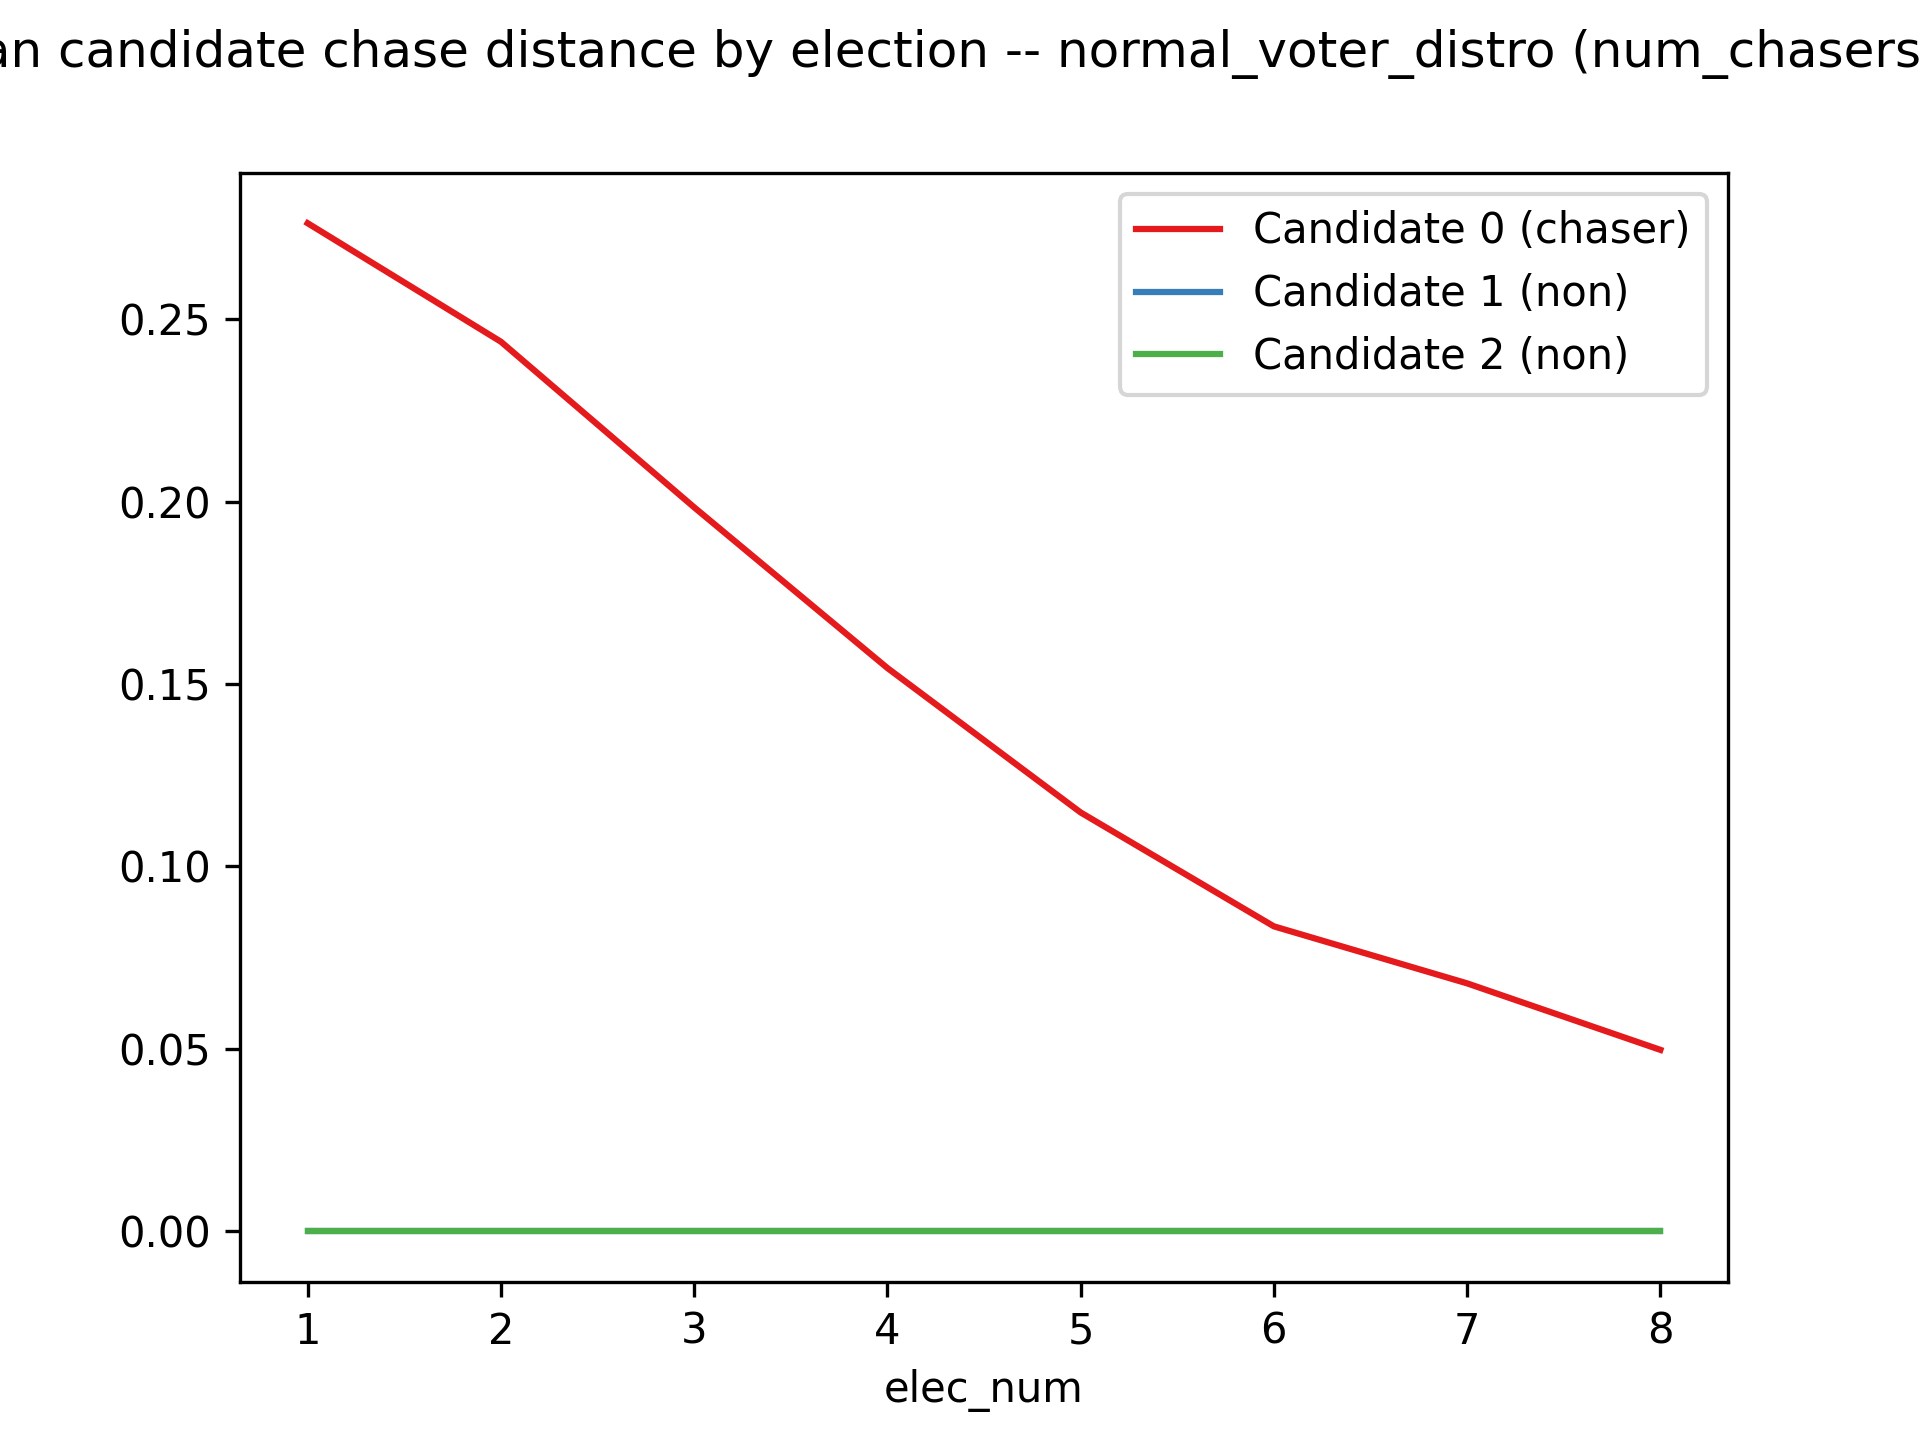
\includegraphics[width=0.45\textwidth]{assets/one_chaser_maxes_out_soon.png}
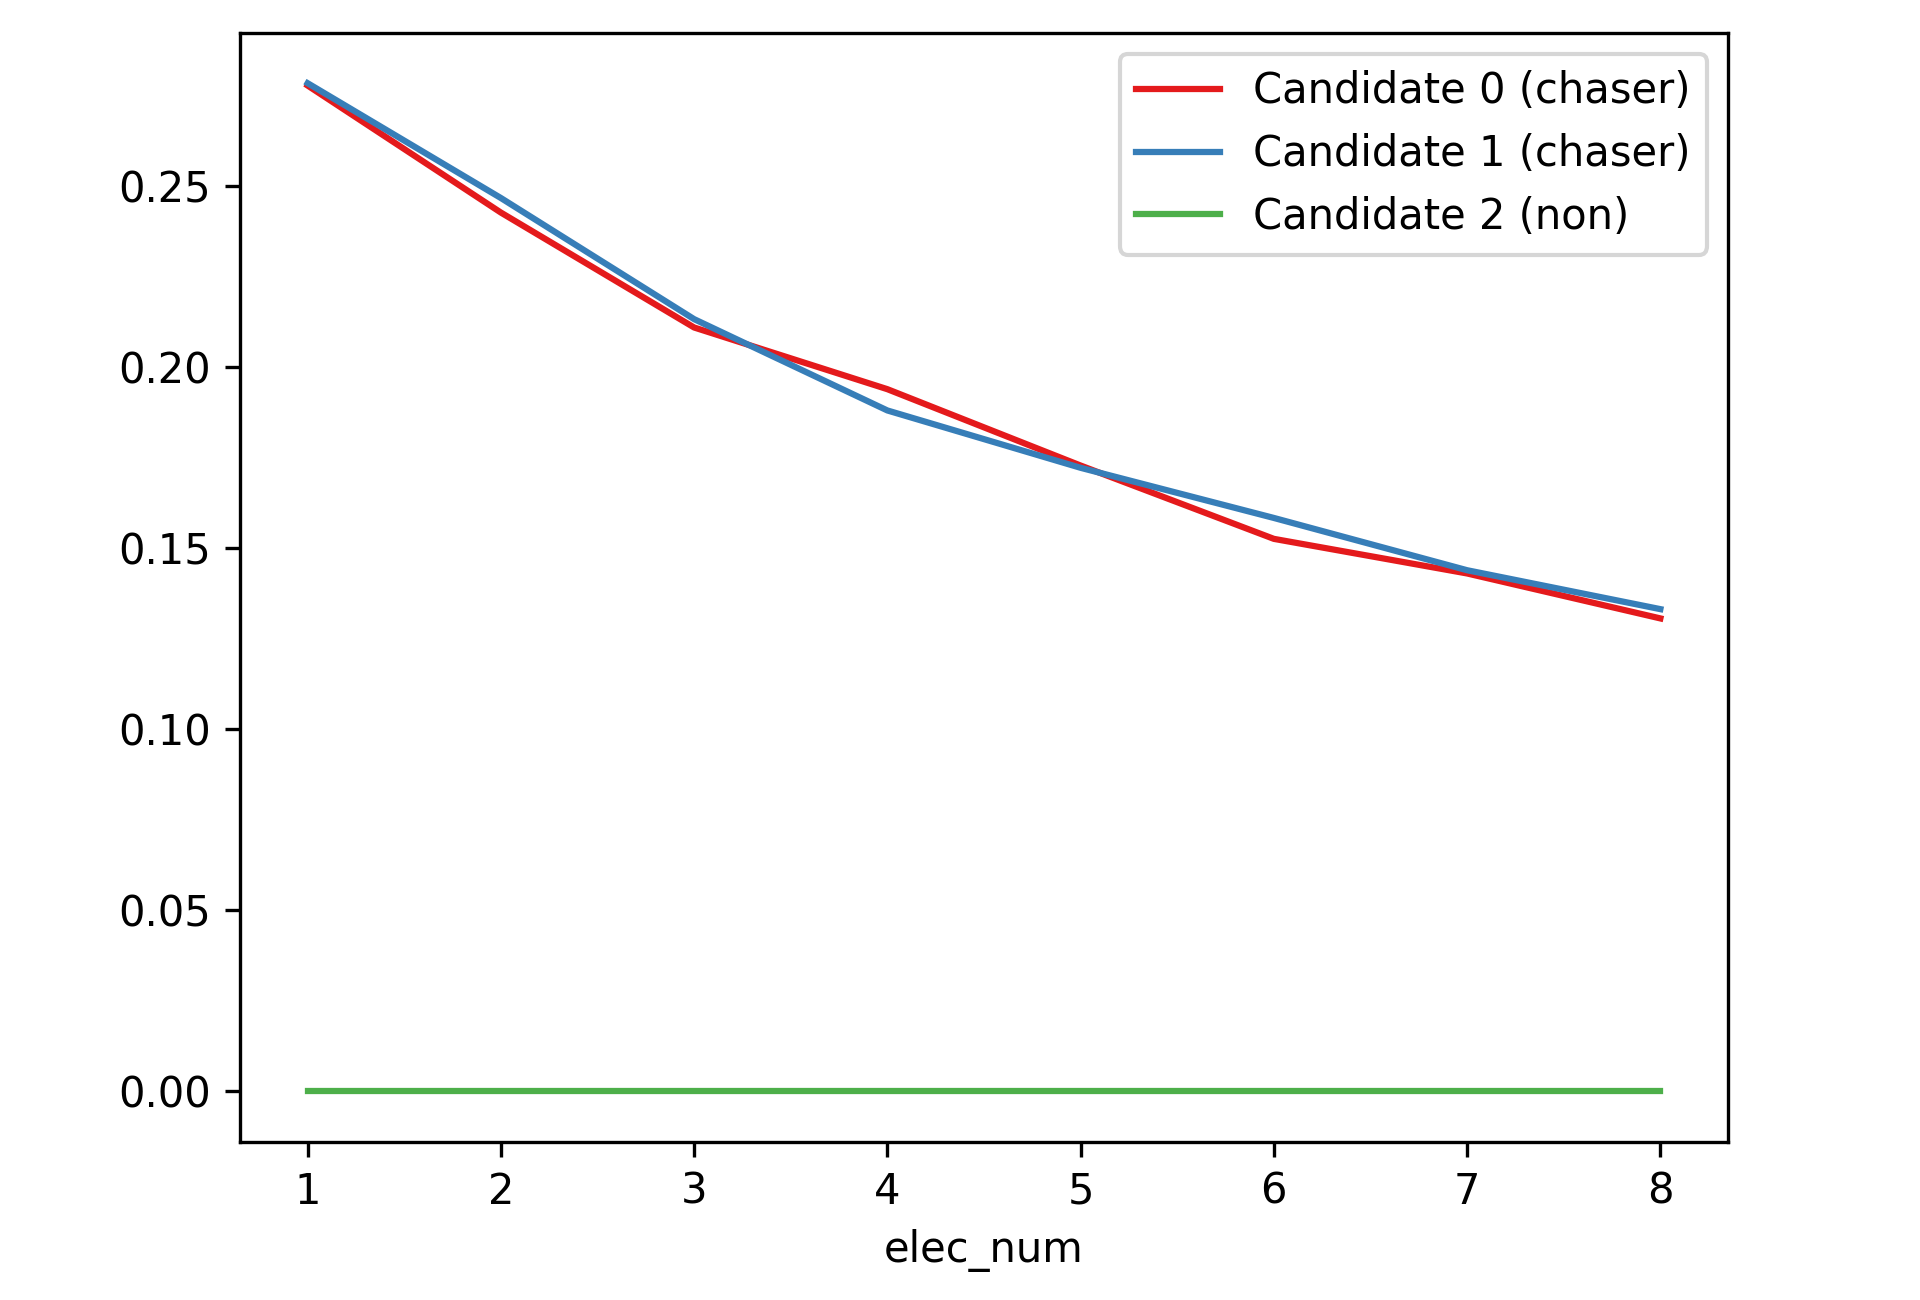
\includegraphics[width=0.45\textwidth]{assets/two_chasers_max_out_later.png}
\caption{A single chasing candidate maxes out its gains more quickly than two
competing chasers do.}
\label{one_vs_two_chasers}
\end{figure}

\subsection{Multiple chasers reduce one another's gains}

The above effect can be further illustrated by looking at how many elections
are actually won by chasing vs. non-chasing candidates.
Figure~\ref{chasing_winners} shows the proportion of elections won by each
candidate in a three-candidate race with one chaser (left side) and with two
(right side). (Error bars are 95\% confidence intervals for a proportion,
assuming normality.) As you can see, when only one candidate chases voters, it
has a tremendous advantage over the other candidates, and this advantage
increases the longer that the drifting/chasing mechanism continues. Two
chasers, however, interfere with one another such that each gets only a modest
benefit.

\begin{figure}[ht]
\centering
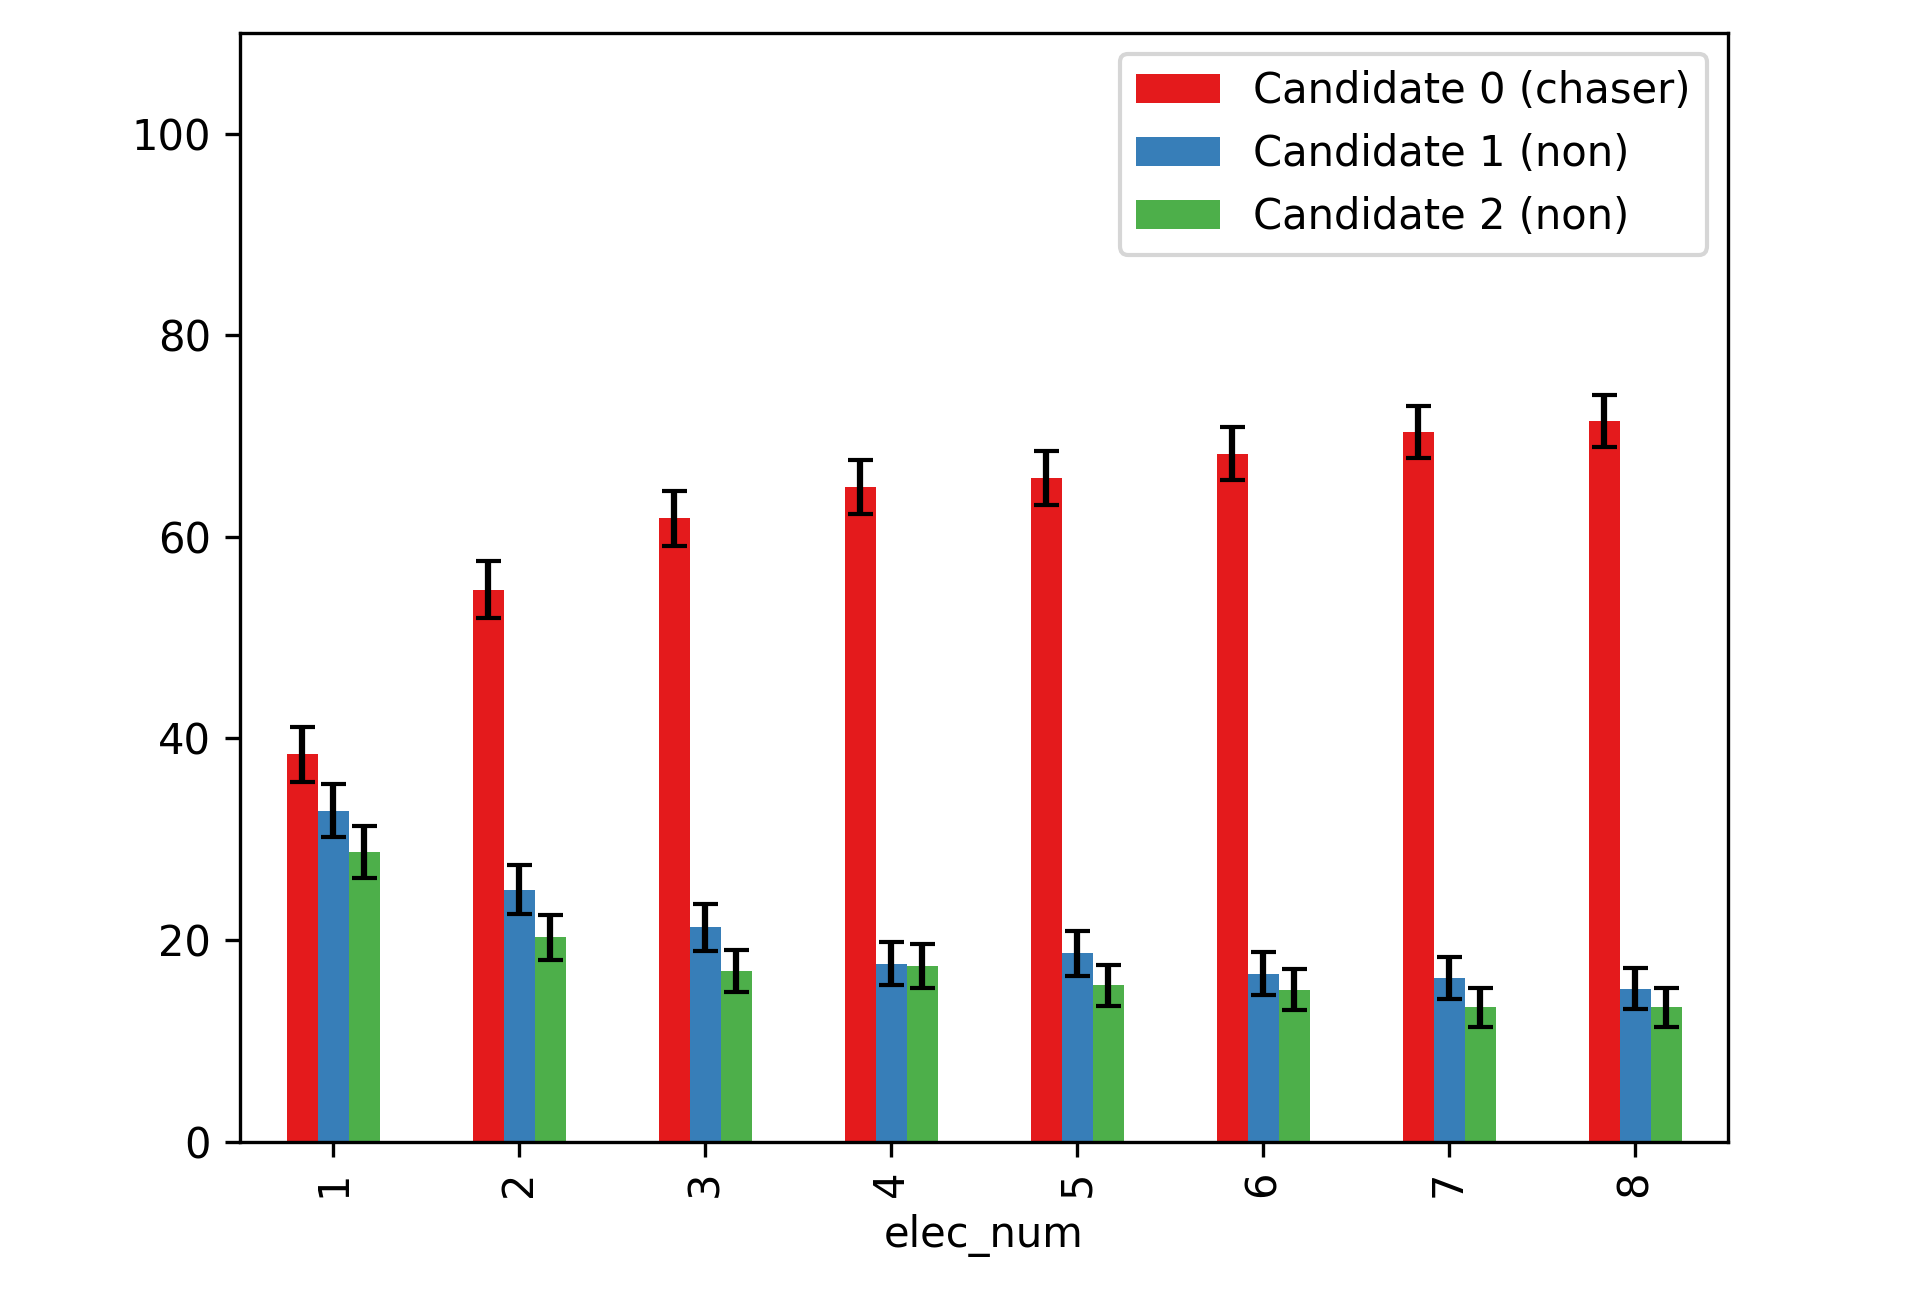
\includegraphics[width=0.45\textwidth]{assets/one_chaser_big_benefit.png}
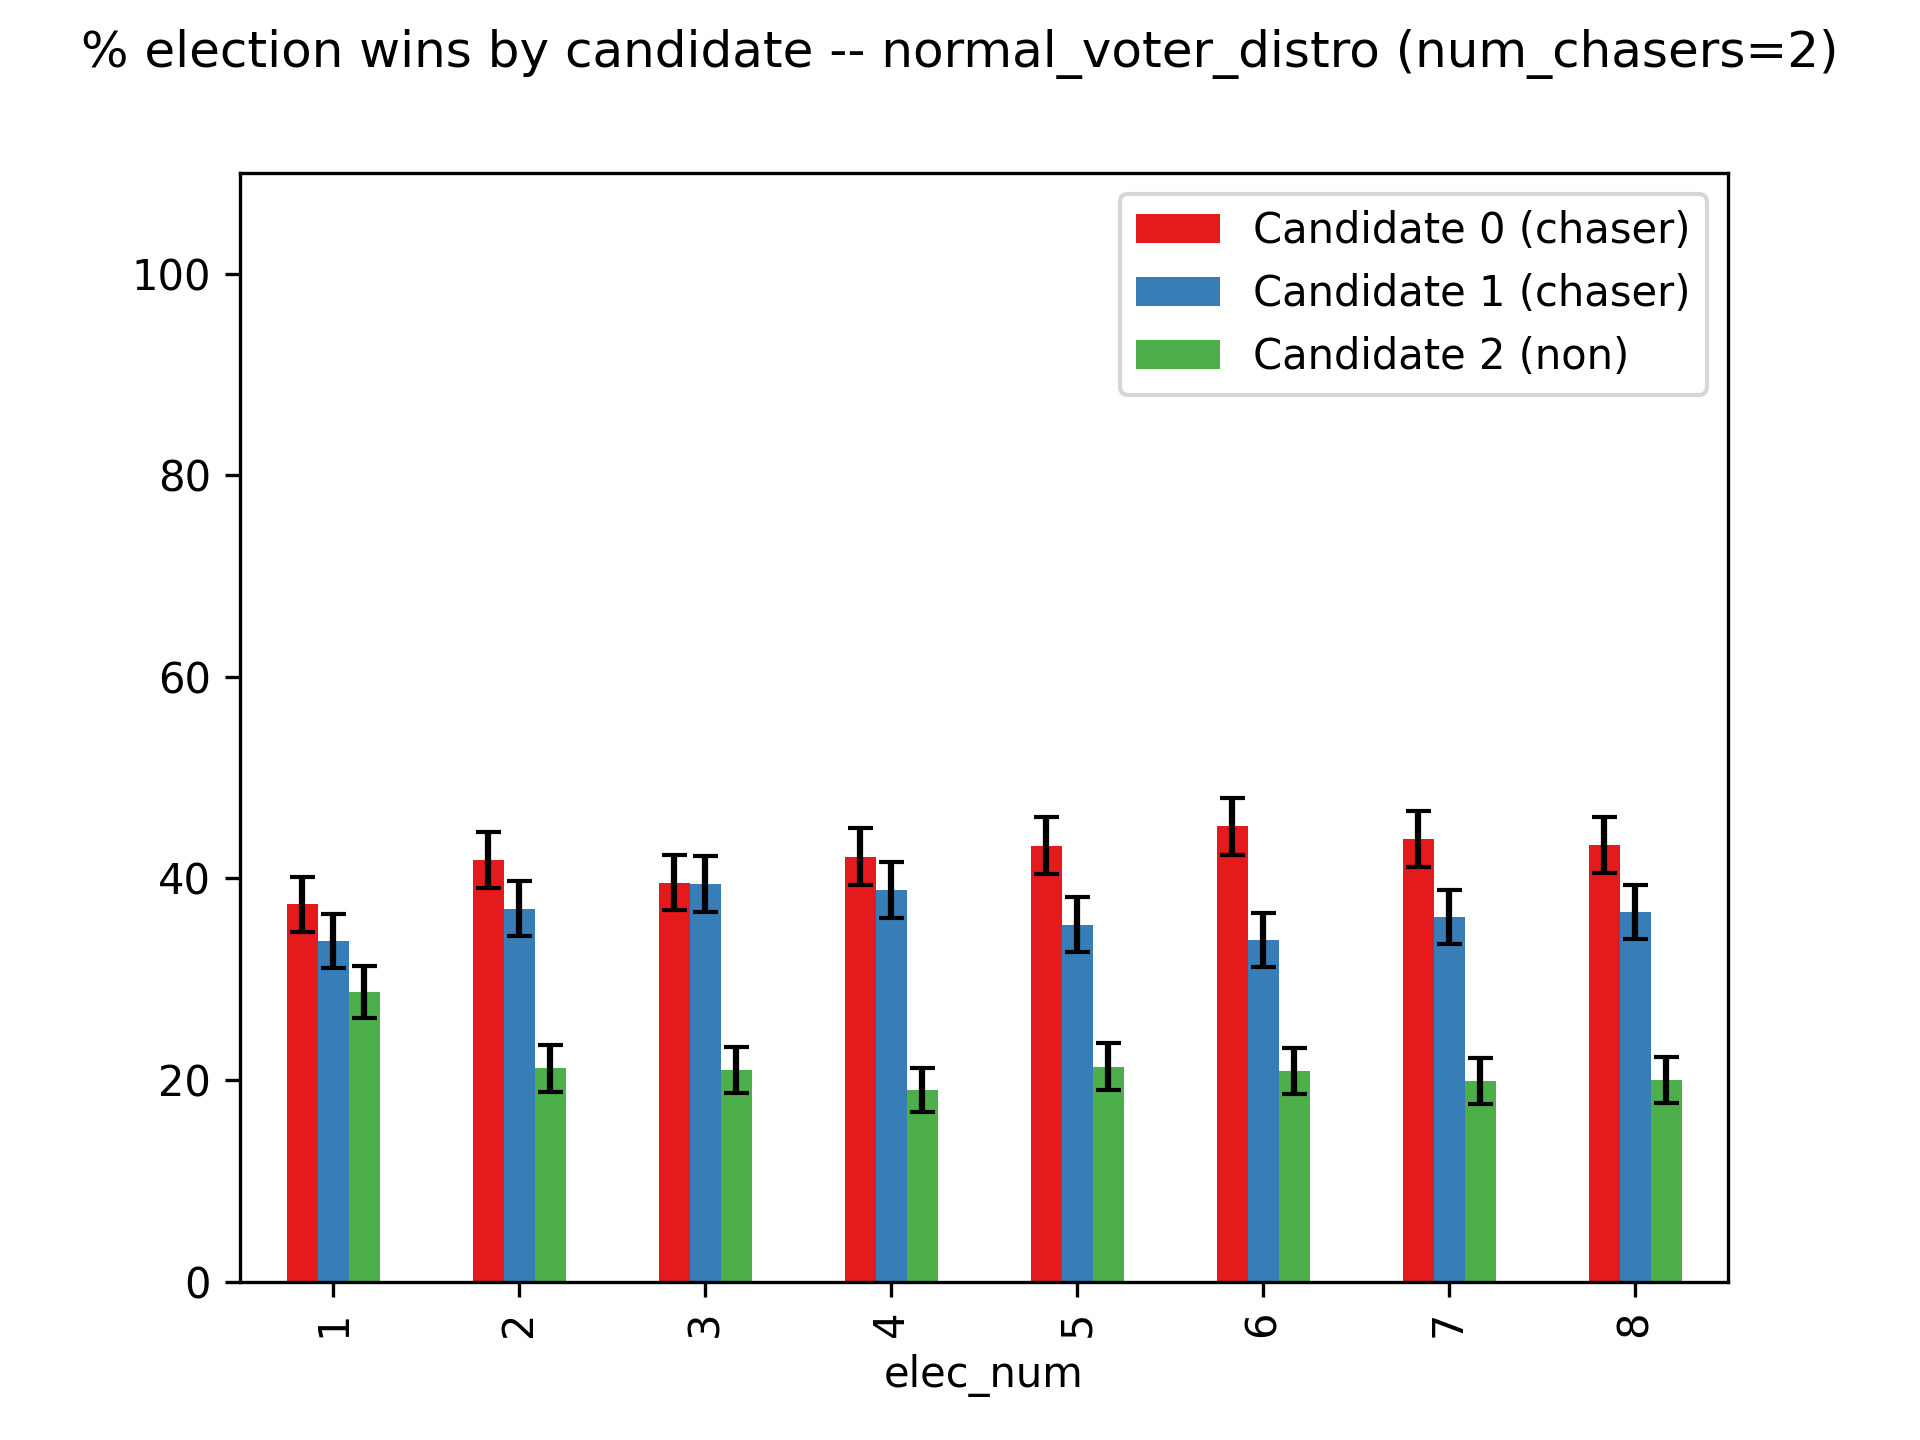
\includegraphics[width=0.45\textwidth]{assets/two_chasers_small_benefit.png}
\caption{Using the default voting algorithm distribution, a single chasing
candidate (red) has an enormous advantage over its competitors. If two
candidates (both red and blue) are chasing voters, however, neither gains
nearly as much benefit. (Note: the small advantages that red consistently has
over blue are an artifact of how the simulation handles ties -- it awards
victory to the lowest-numbered tied candidate. This is miniscule in comparison
with the main effect illustrated here, however.)}
\label{chasing_winners}
\end{figure}

\subsection{The impact of voting algorithm distribution}

All of the above results were obtained with the default voting algorithm
distribution ($\frac{1}{3}$ rational, $\frac{1}{3}$ party, $\frac{1}{6}$ F\&F1,
$\frac{1}{6}$ F\&F2) and it turns out they are highly sensitive to it. In an
electorate with \textit{no} rational voters, by contrast, chasers get little to
no benefit. They are trying to appeal to the issue positions of voters who will
not in fact be voting based on those positions. Chasing candidates have no
advantage even if there are many, or even all, F\&F voters. This is somewhat
surprising since F\&F voters do ``noisily'' vote based on their issue positions
(they consider only one of them, instead of all three). Compare
Figure~\ref{chasing_vs_distro} (the left side has all party-line voters, the
right side has all F\&F voters) with the left side of
Figure~\ref{chasing_winners} (which has the default voting algorithm
distribution) to see the difference.

\begin{figure}[ht]
\centering
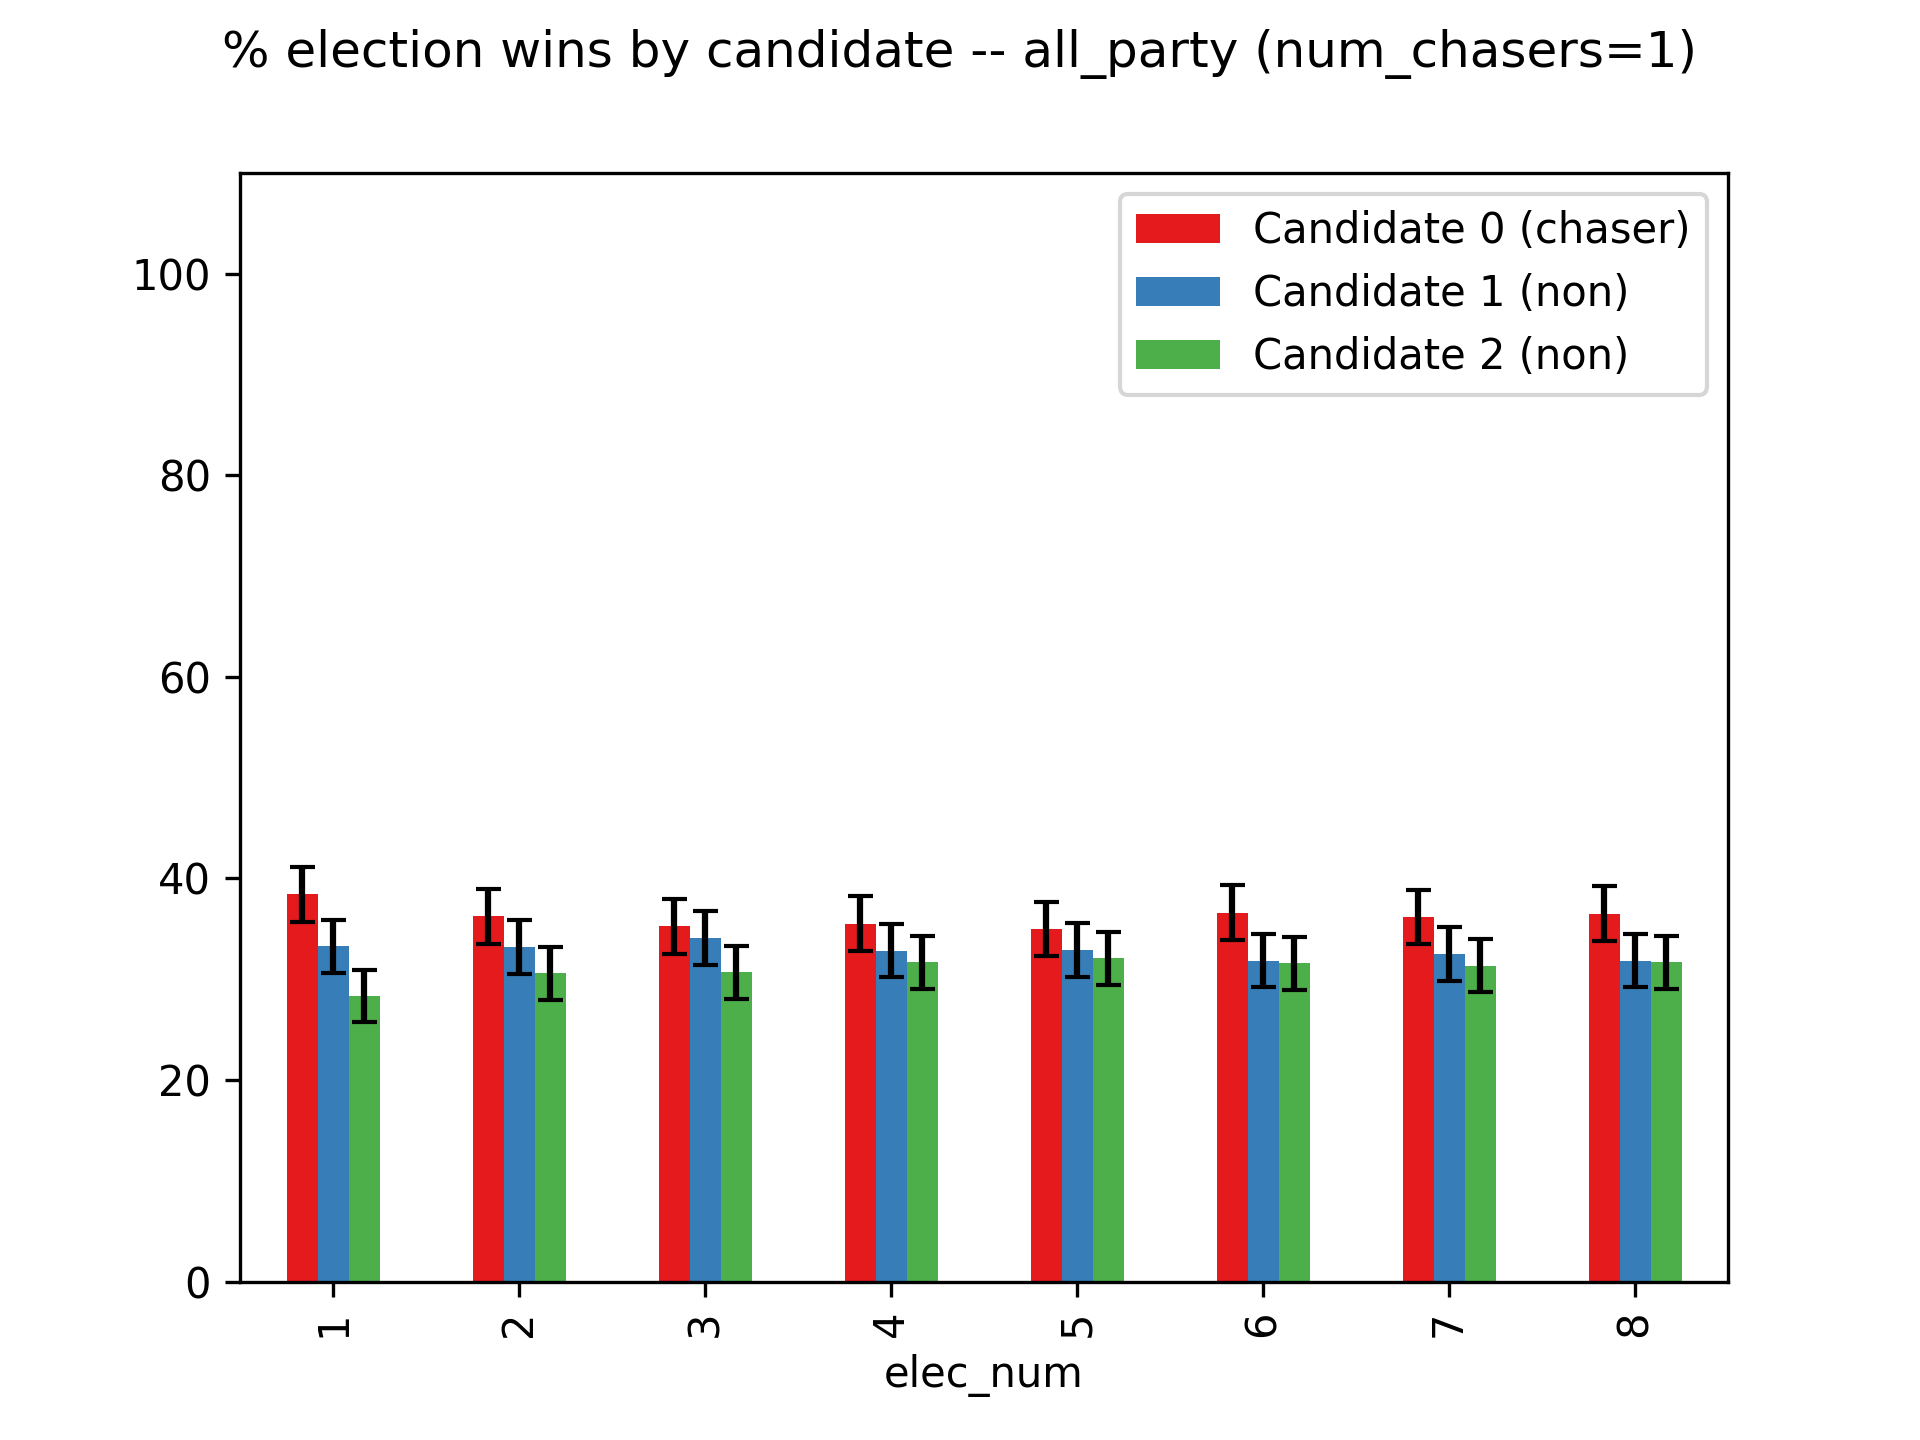
\includegraphics[width=0.45\textwidth]{assets/all_party_1_chaser_no_benefit.png}
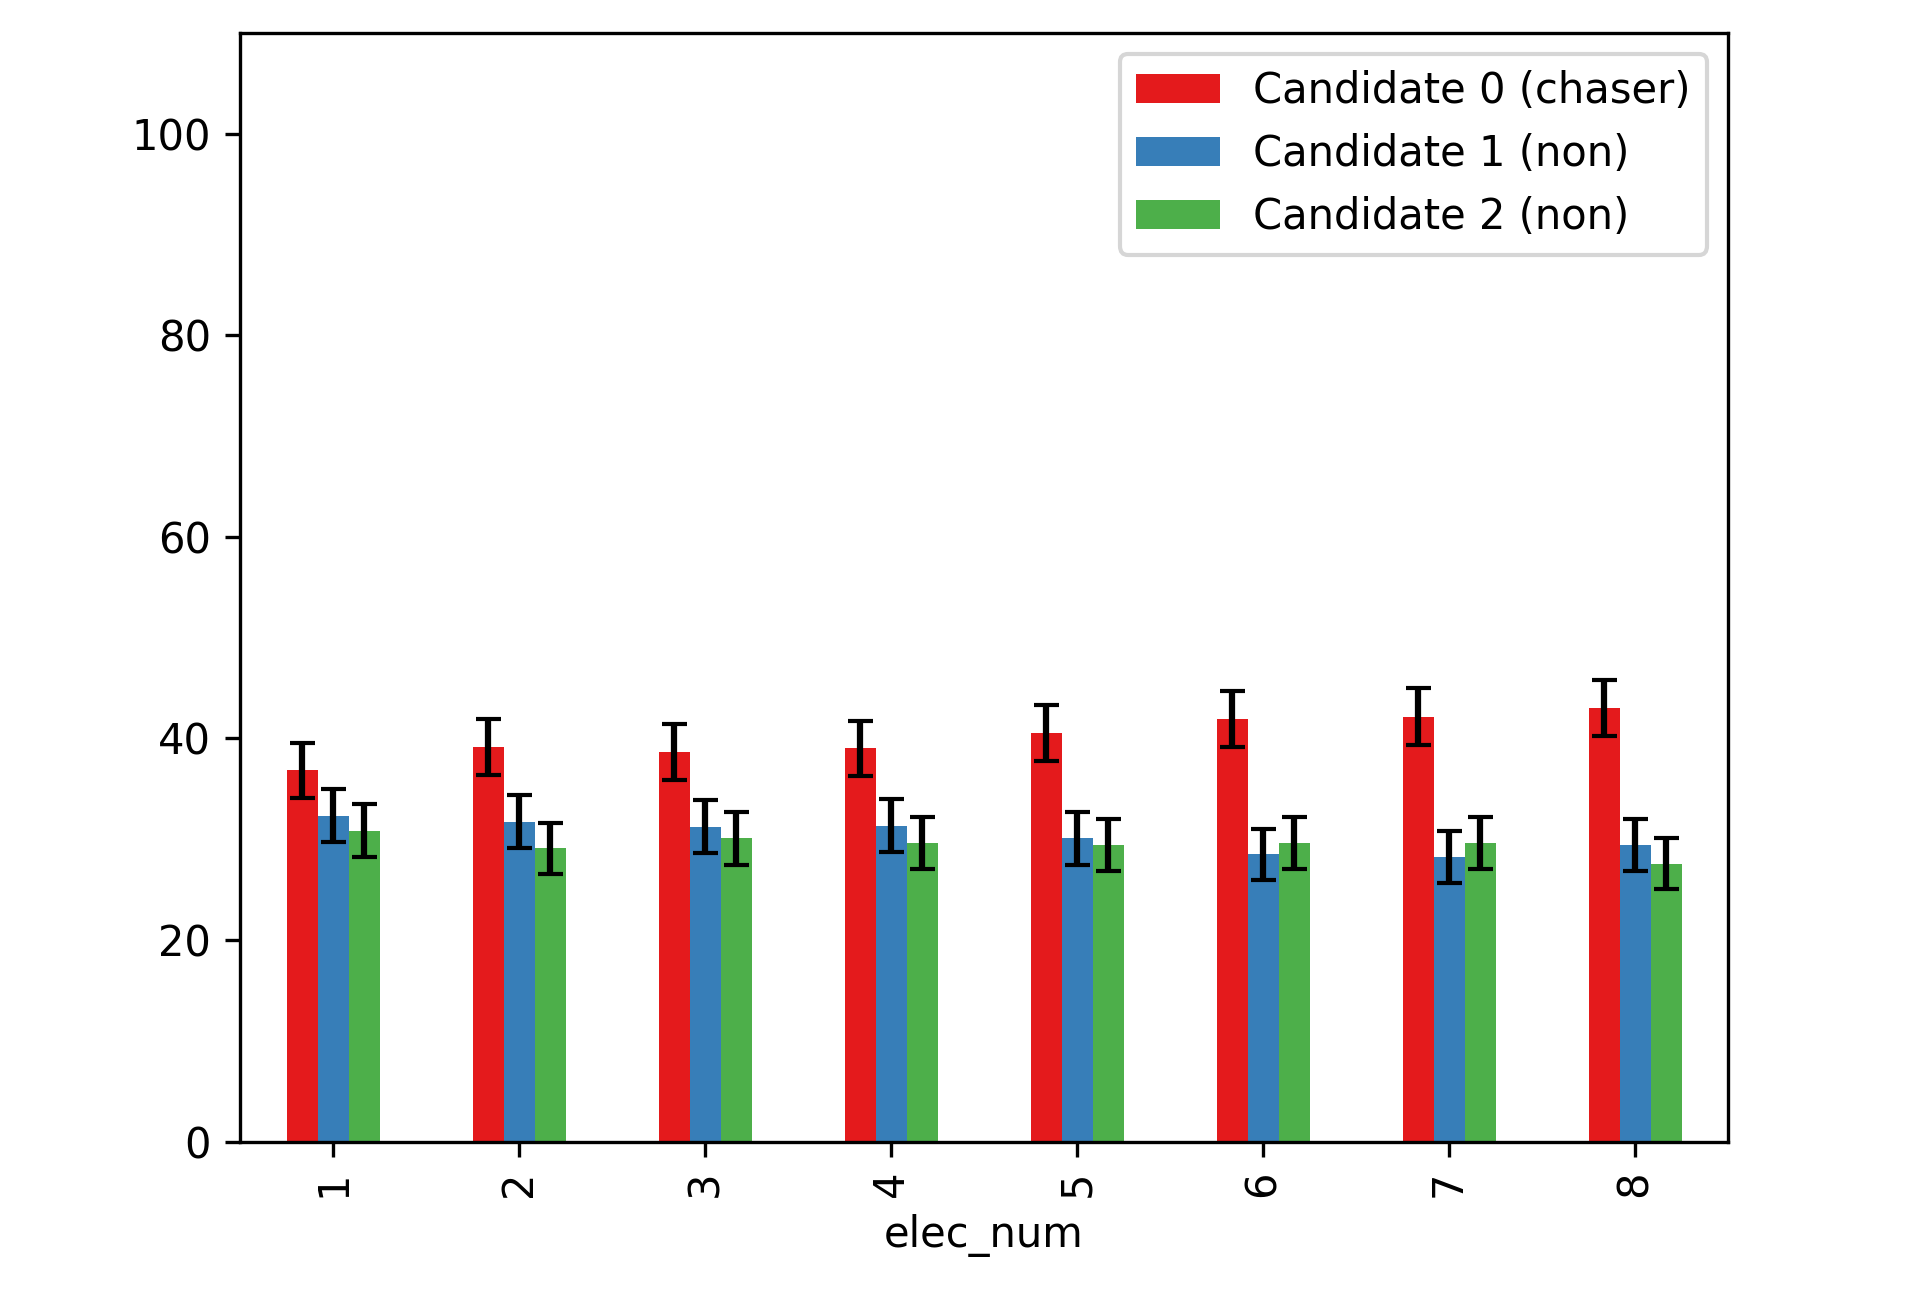
\includegraphics[width=0.45\textwidth]{assets/all_ff_chasers_no_benefit.png}
\caption{When the electorate is changed to have all party-line voters (left) or
all fast \& frugal voters (right), chasing candidates have little appreciable
advantage.}
\label{chasing_vs_distro}
\end{figure}

At the other extreme, an electorate of all rational voters gives the maximum
benefit to chasing candidates (see Figure~\ref{all_rat_chasers_benefit}). In
this scenario, even when two candidates are chasers, they do not interfere with
one another enough to nullify their effects -- both easily eclipse the single
non-chasing candidate (Figure~\ref{all_rat_chasers_benefit}, right side.)

\begin{figure}[ht]
\centering
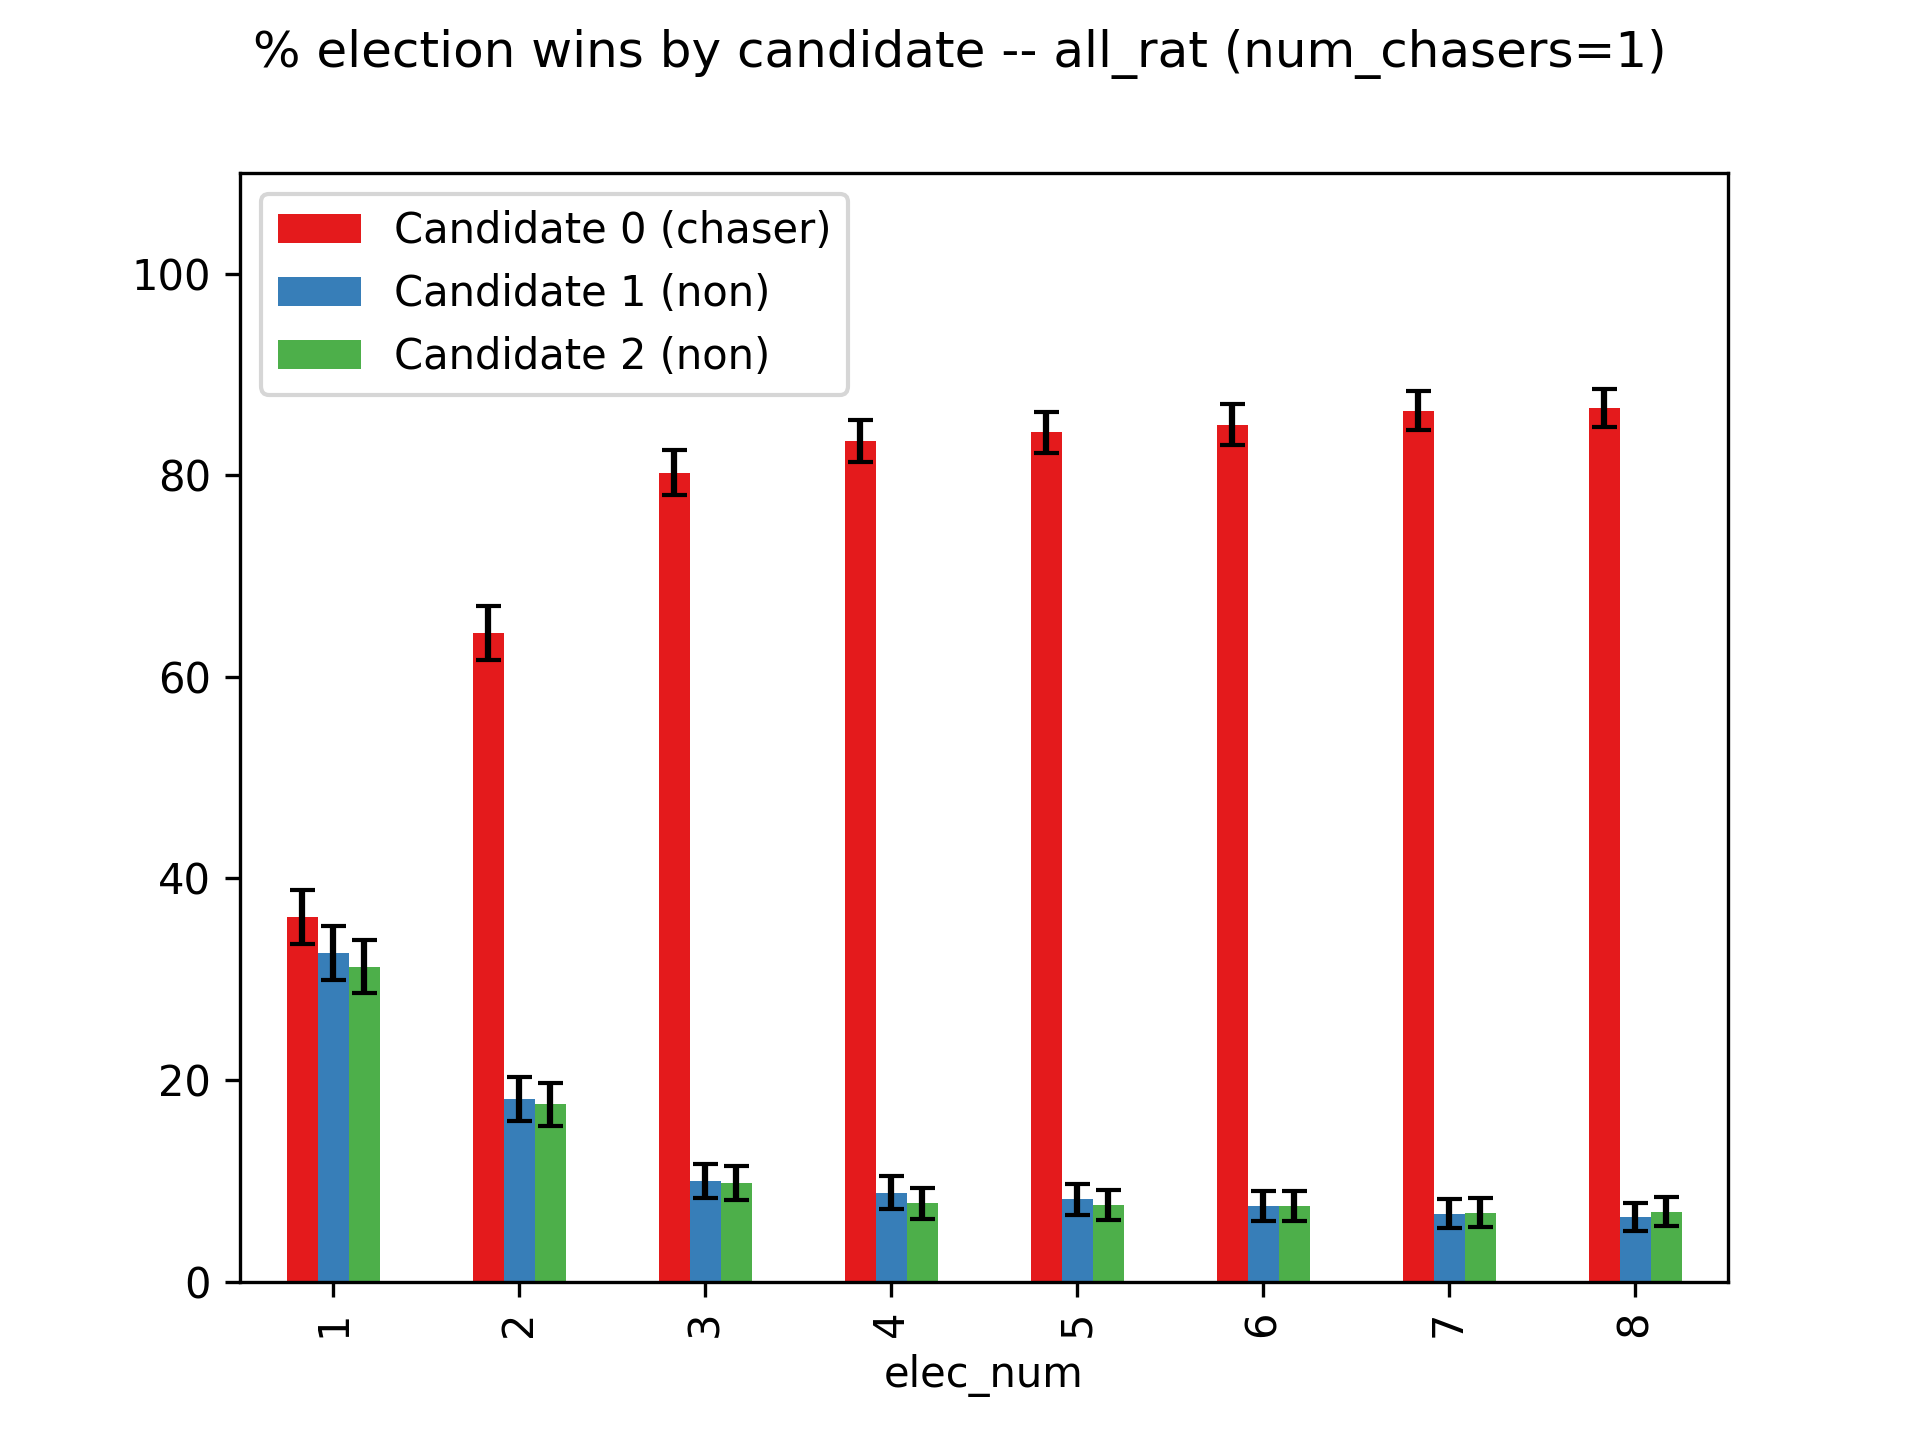
\includegraphics[width=0.45\textwidth]{assets/all_rat_one_chaser_even_bigger_benefit.png}
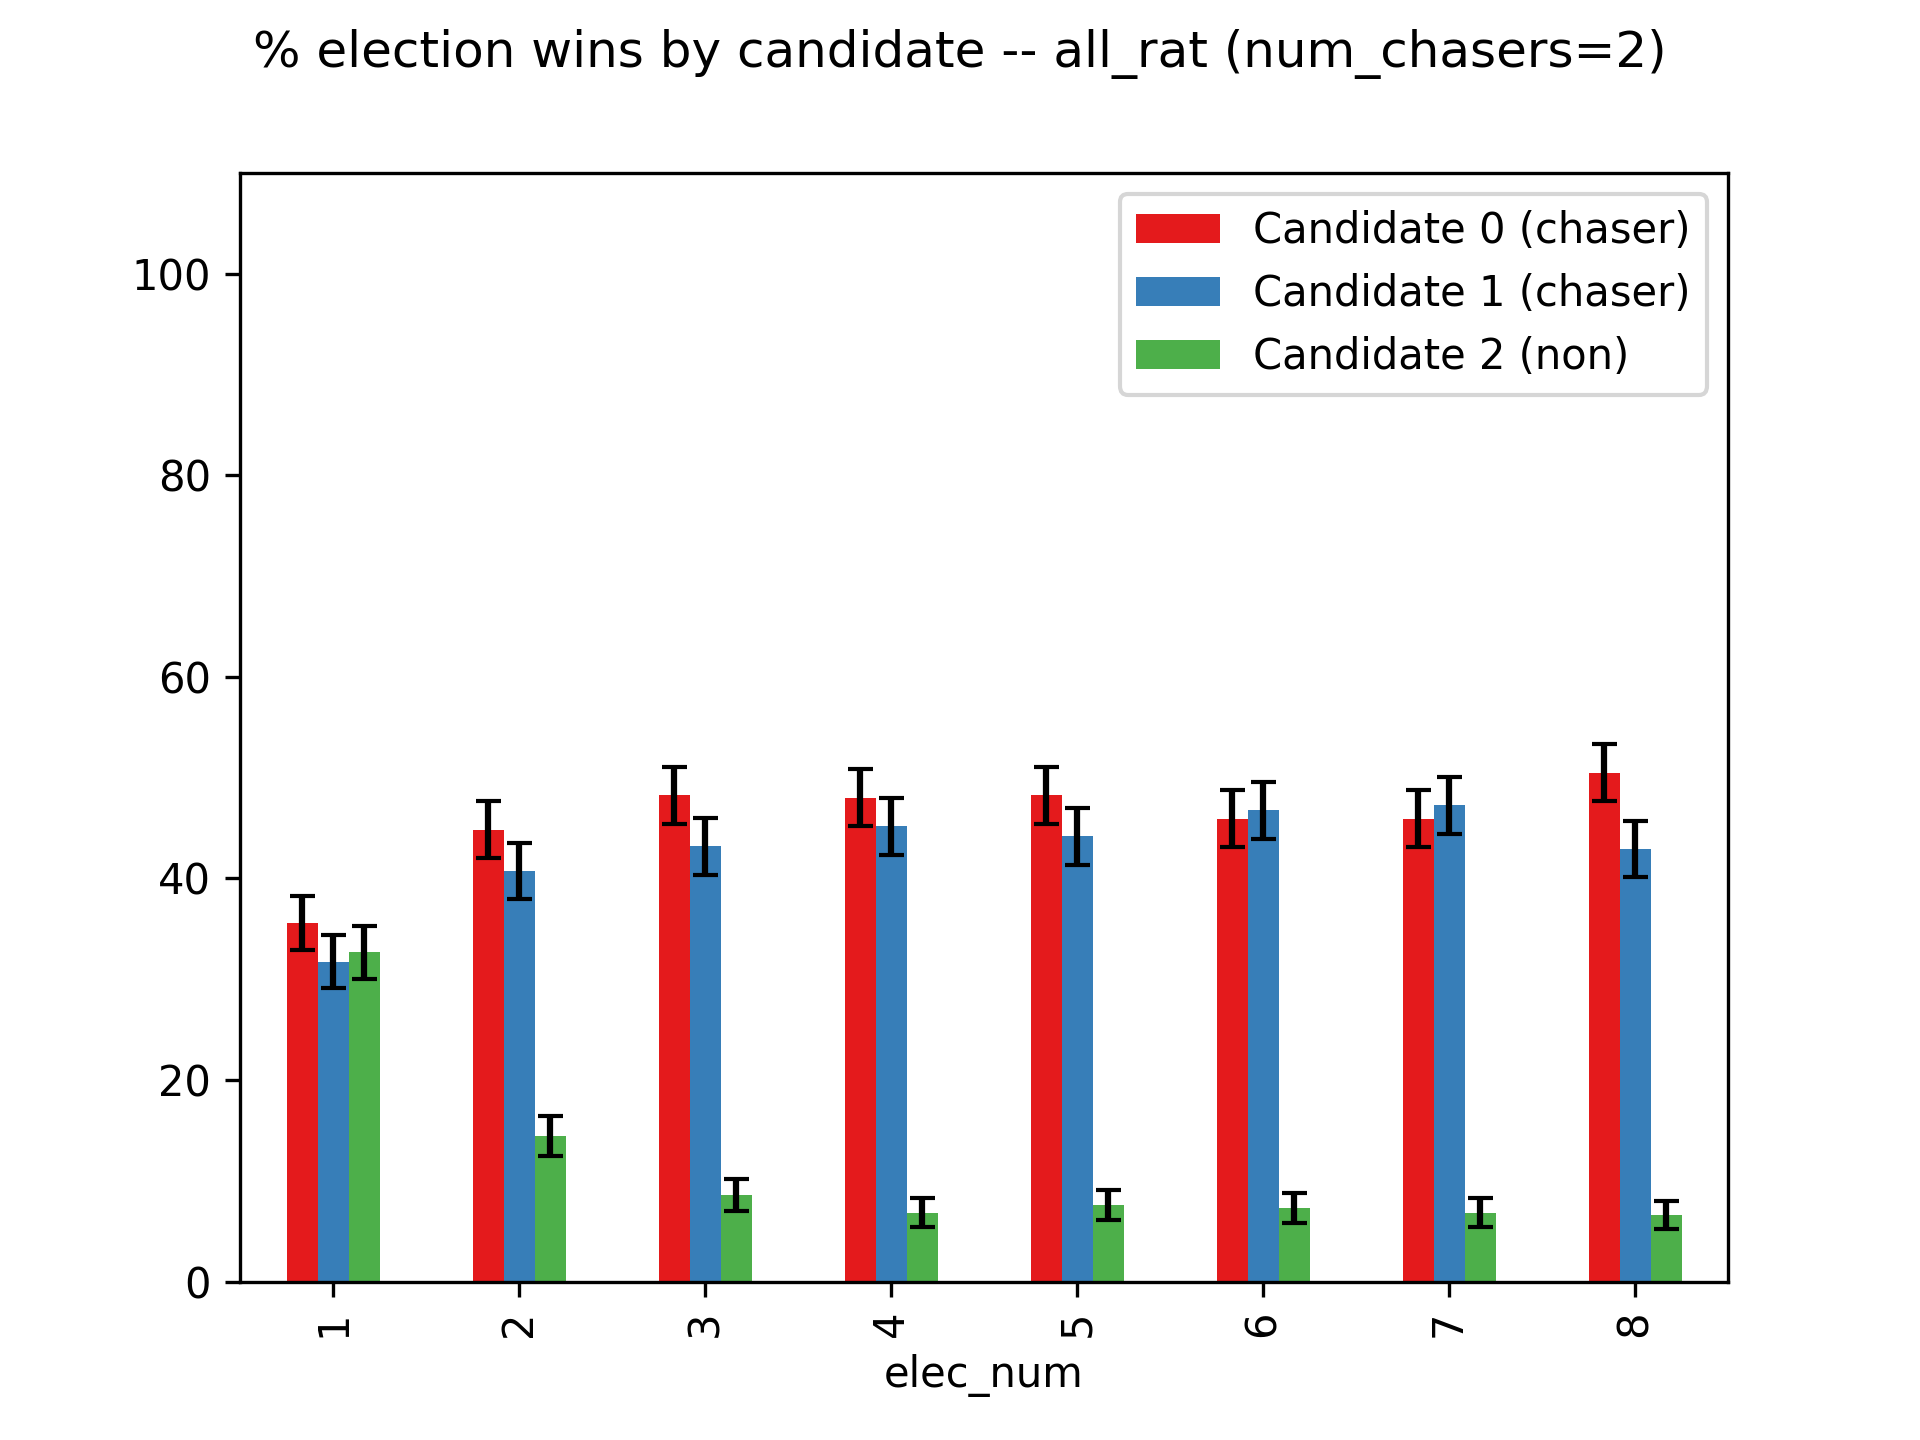
\includegraphics[width=0.45\textwidth]{assets/all_rat_two_chasers_even_bigger_benefit.png}
\caption{An electorate of all rational voters confers maximum benefit to
chasing. Even when there are two chasers (right side) they each receive an
advantage.}
\label{all_rat_chasers_benefit}
\end{figure}


\subsection{The rationality of election outcomes}

Now, using an electorate of all party-line voters, we can measure the impact of
blind party voters on the rationality of election outcomes. An election is considered 
rational if the candidate who actually wins is the same candidate who would have 
won if all agents had voted rationally.
 
Despite the fact that
party affiliations are in line with voter and candidate opinions, voters'
stubbornness in remaining with their parties, as modeled modestly by the party switch
threshold, becomes detrimental to the rationality of elections.
Figure~\ref{all_party_hurt_rat} (left) shows that when no candidates are chasing votes and all 
agents are party-line voters, approximately 60\% of elections are rational. 

More so, when candidates are chasing party-line voters, not only does it fail to provide an 
advantage (as determined above), but it actually decreases the rationality of elections 
(Figure~\ref{all_party_hurt_rat}, right side).

\begin{figure}
\centering
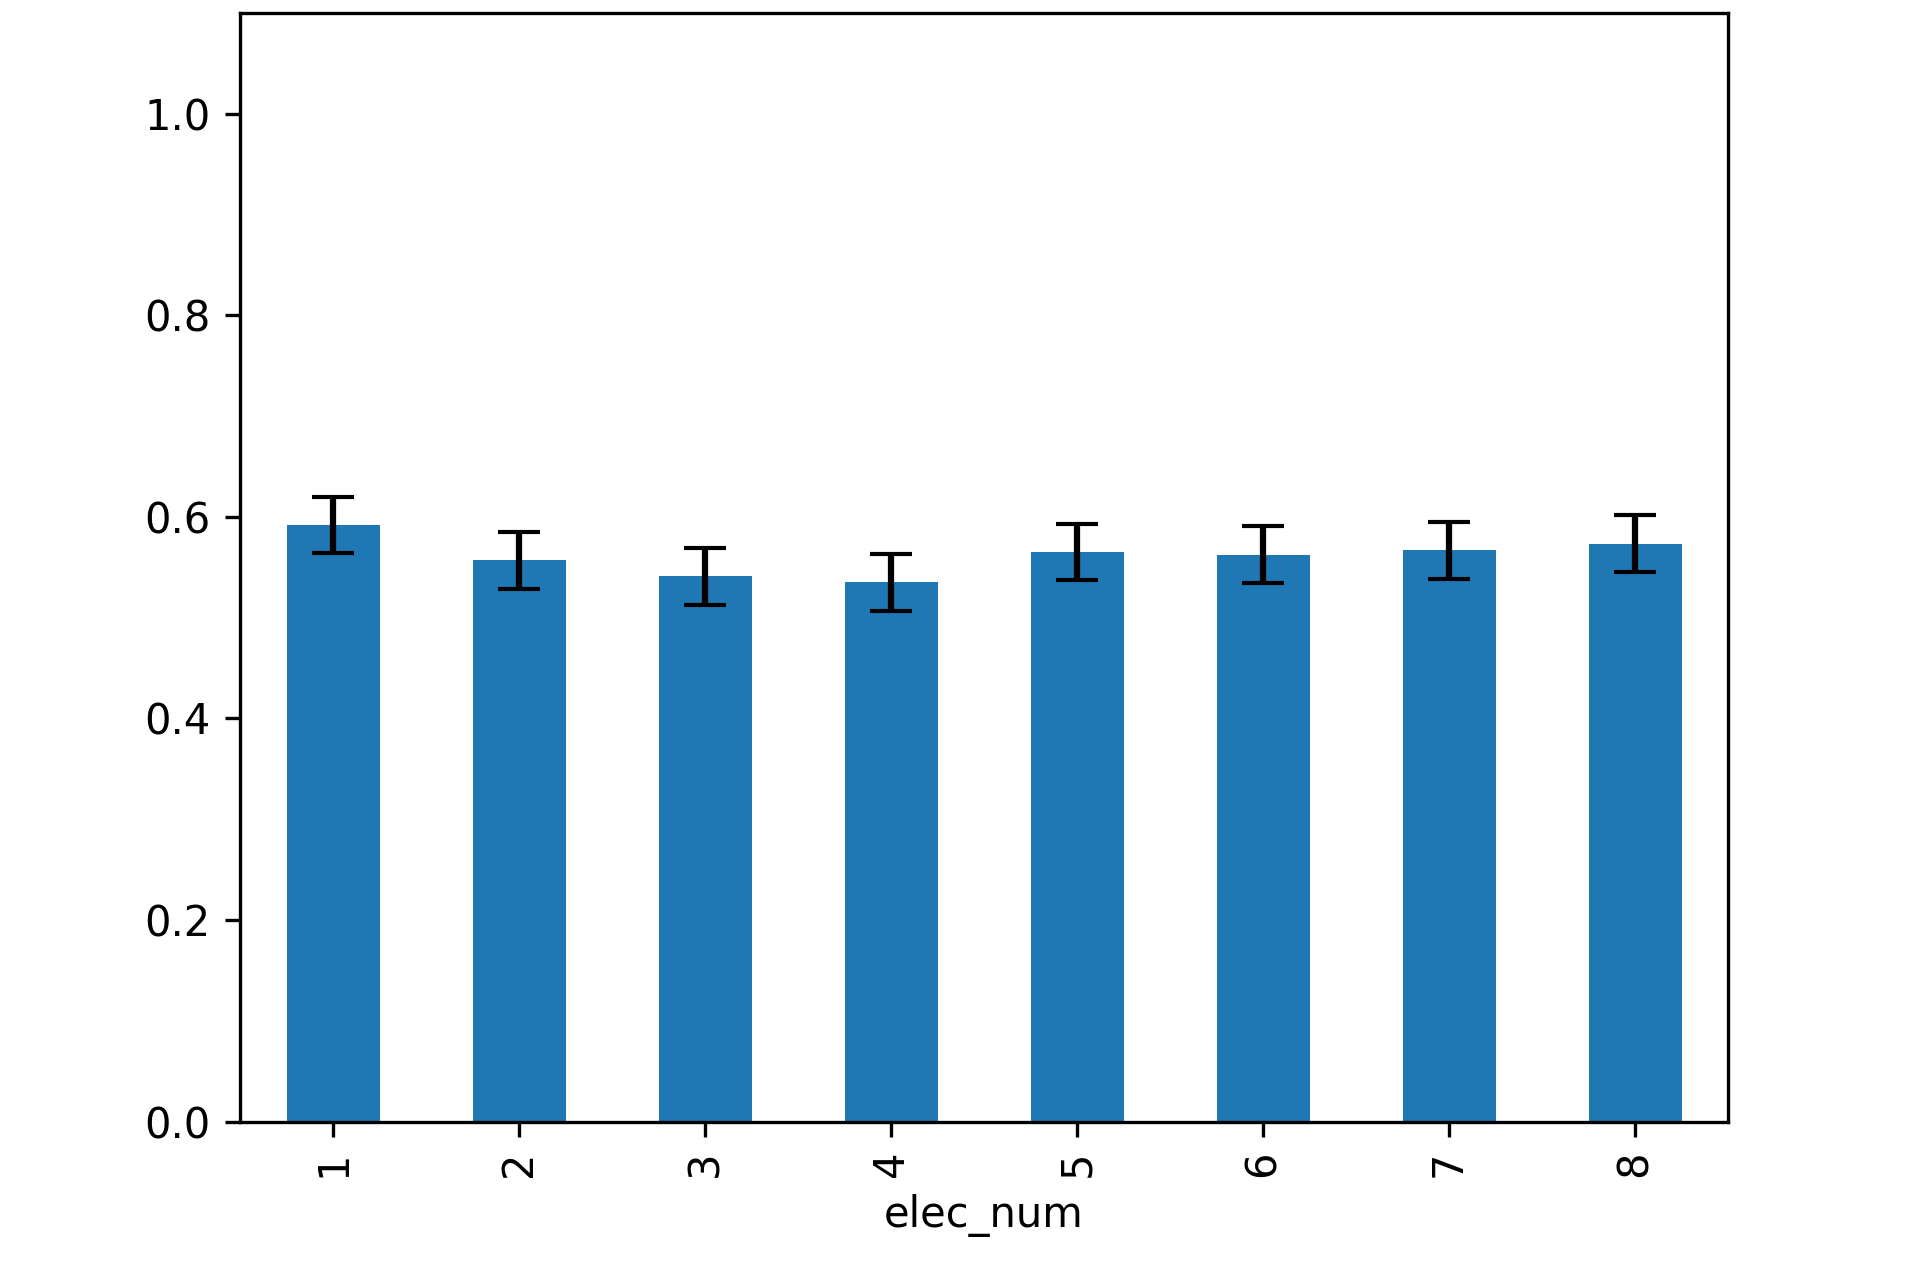
\includegraphics[width=0.45\textwidth]{assets/all_party_0_chasers_rationality_stays_same.png}
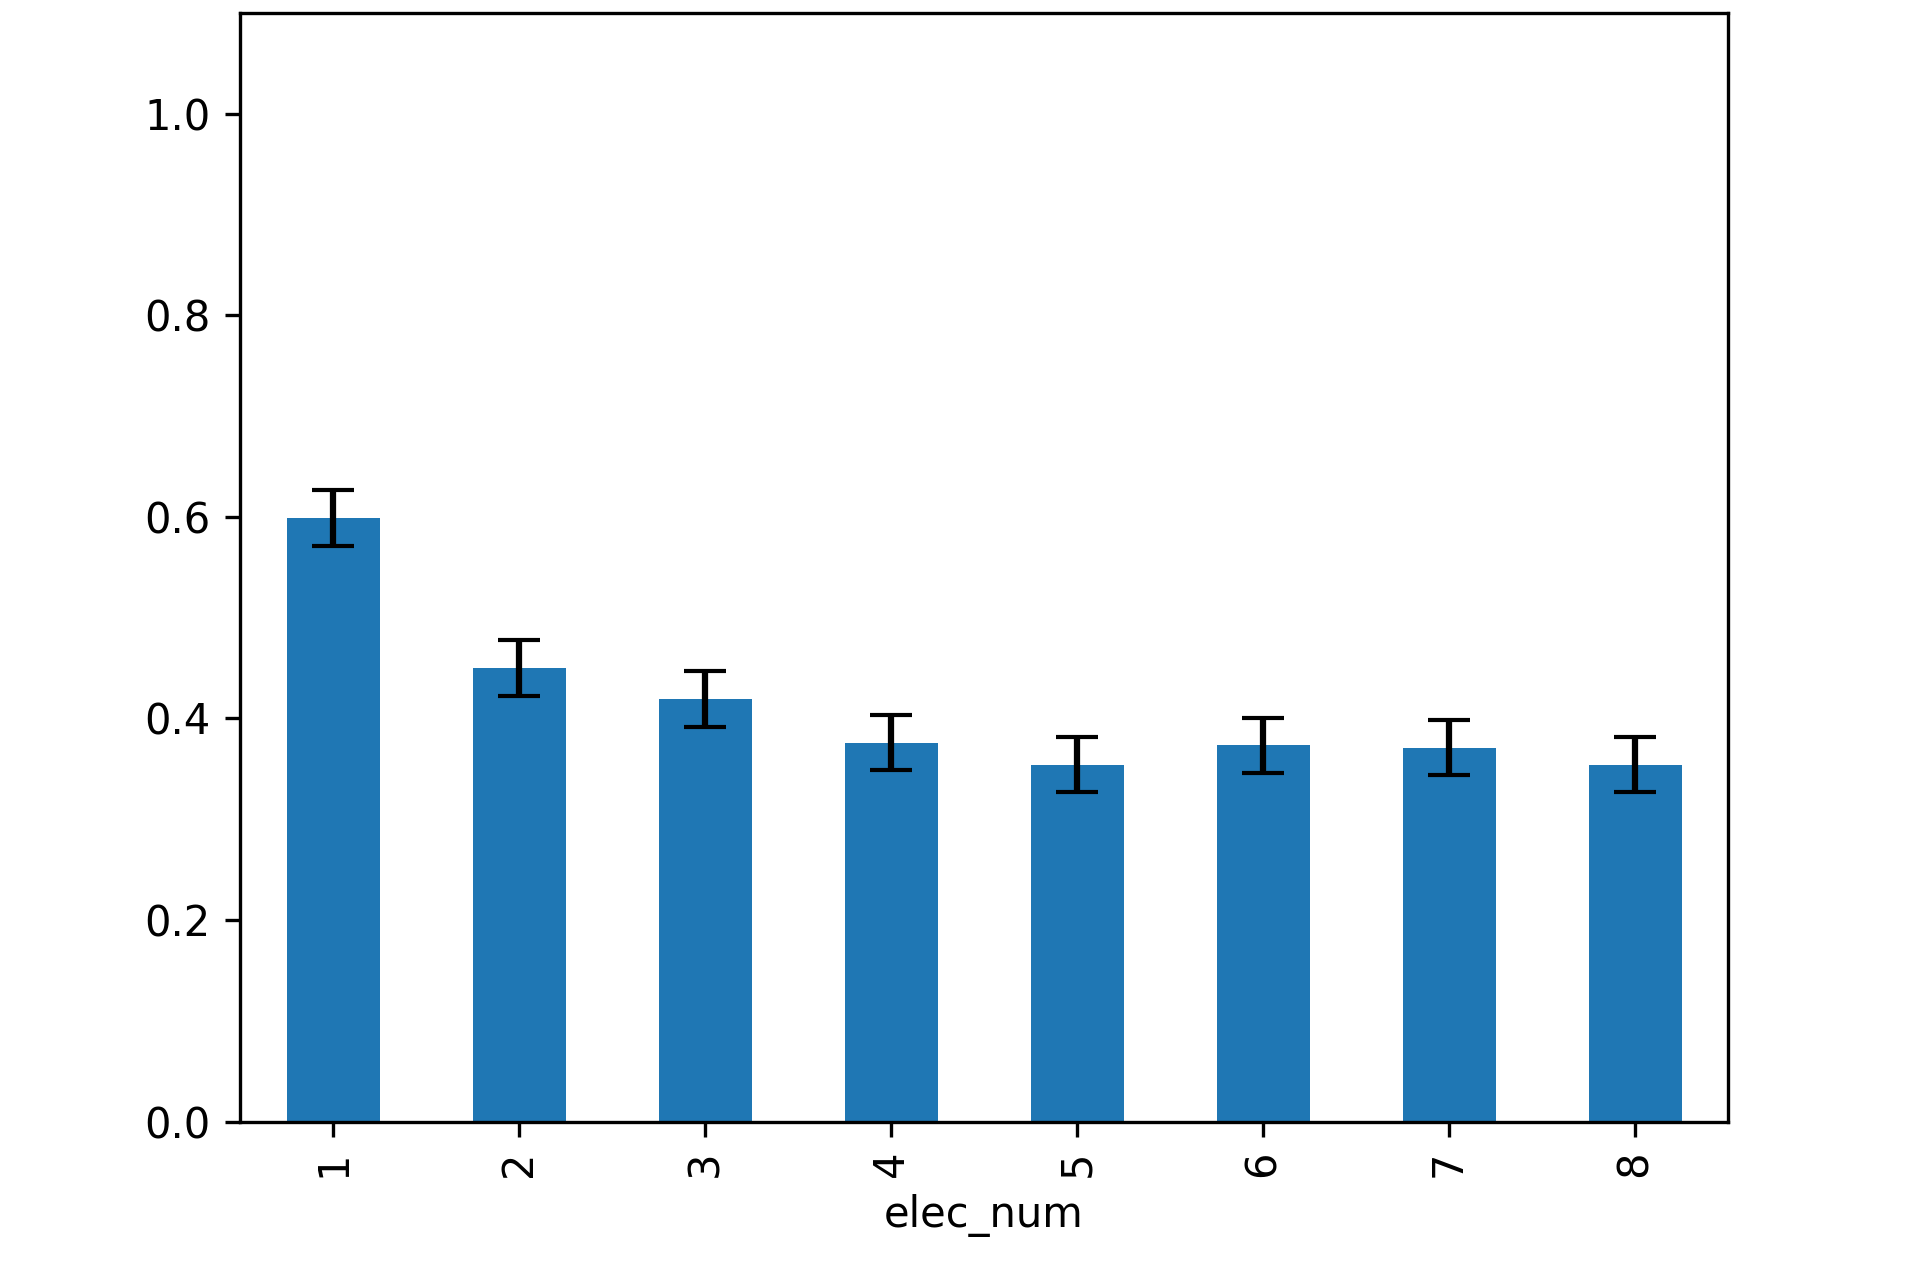
\includegraphics[width=0.45\textwidth]{assets/all_party_3_chasers_rationality_decreases.png}
	\caption{The percentage of rational election outcomes with an electorate of all party-line voters 
	remains constant when there are zero chasing candidates (left), but decreases with three chasing
	candidates (right).}
	\label{all_party_hurt_rat}
\end{figure}


\subsection{The chase radius}

Recall that the chase radius sets a limit on how far candidates can wander in
opinion space every time they chase voters. Interestingly, the value of this
parameter has little effect on election outcomes. Figure~\ref{chase_radius}
shows winner outcomes in two-chaser elections for three different values of the
chase radius (the same value is shared by both chasing candidates): 0.1, 0.2,
and 0.3.

\begin{figure}
\centering
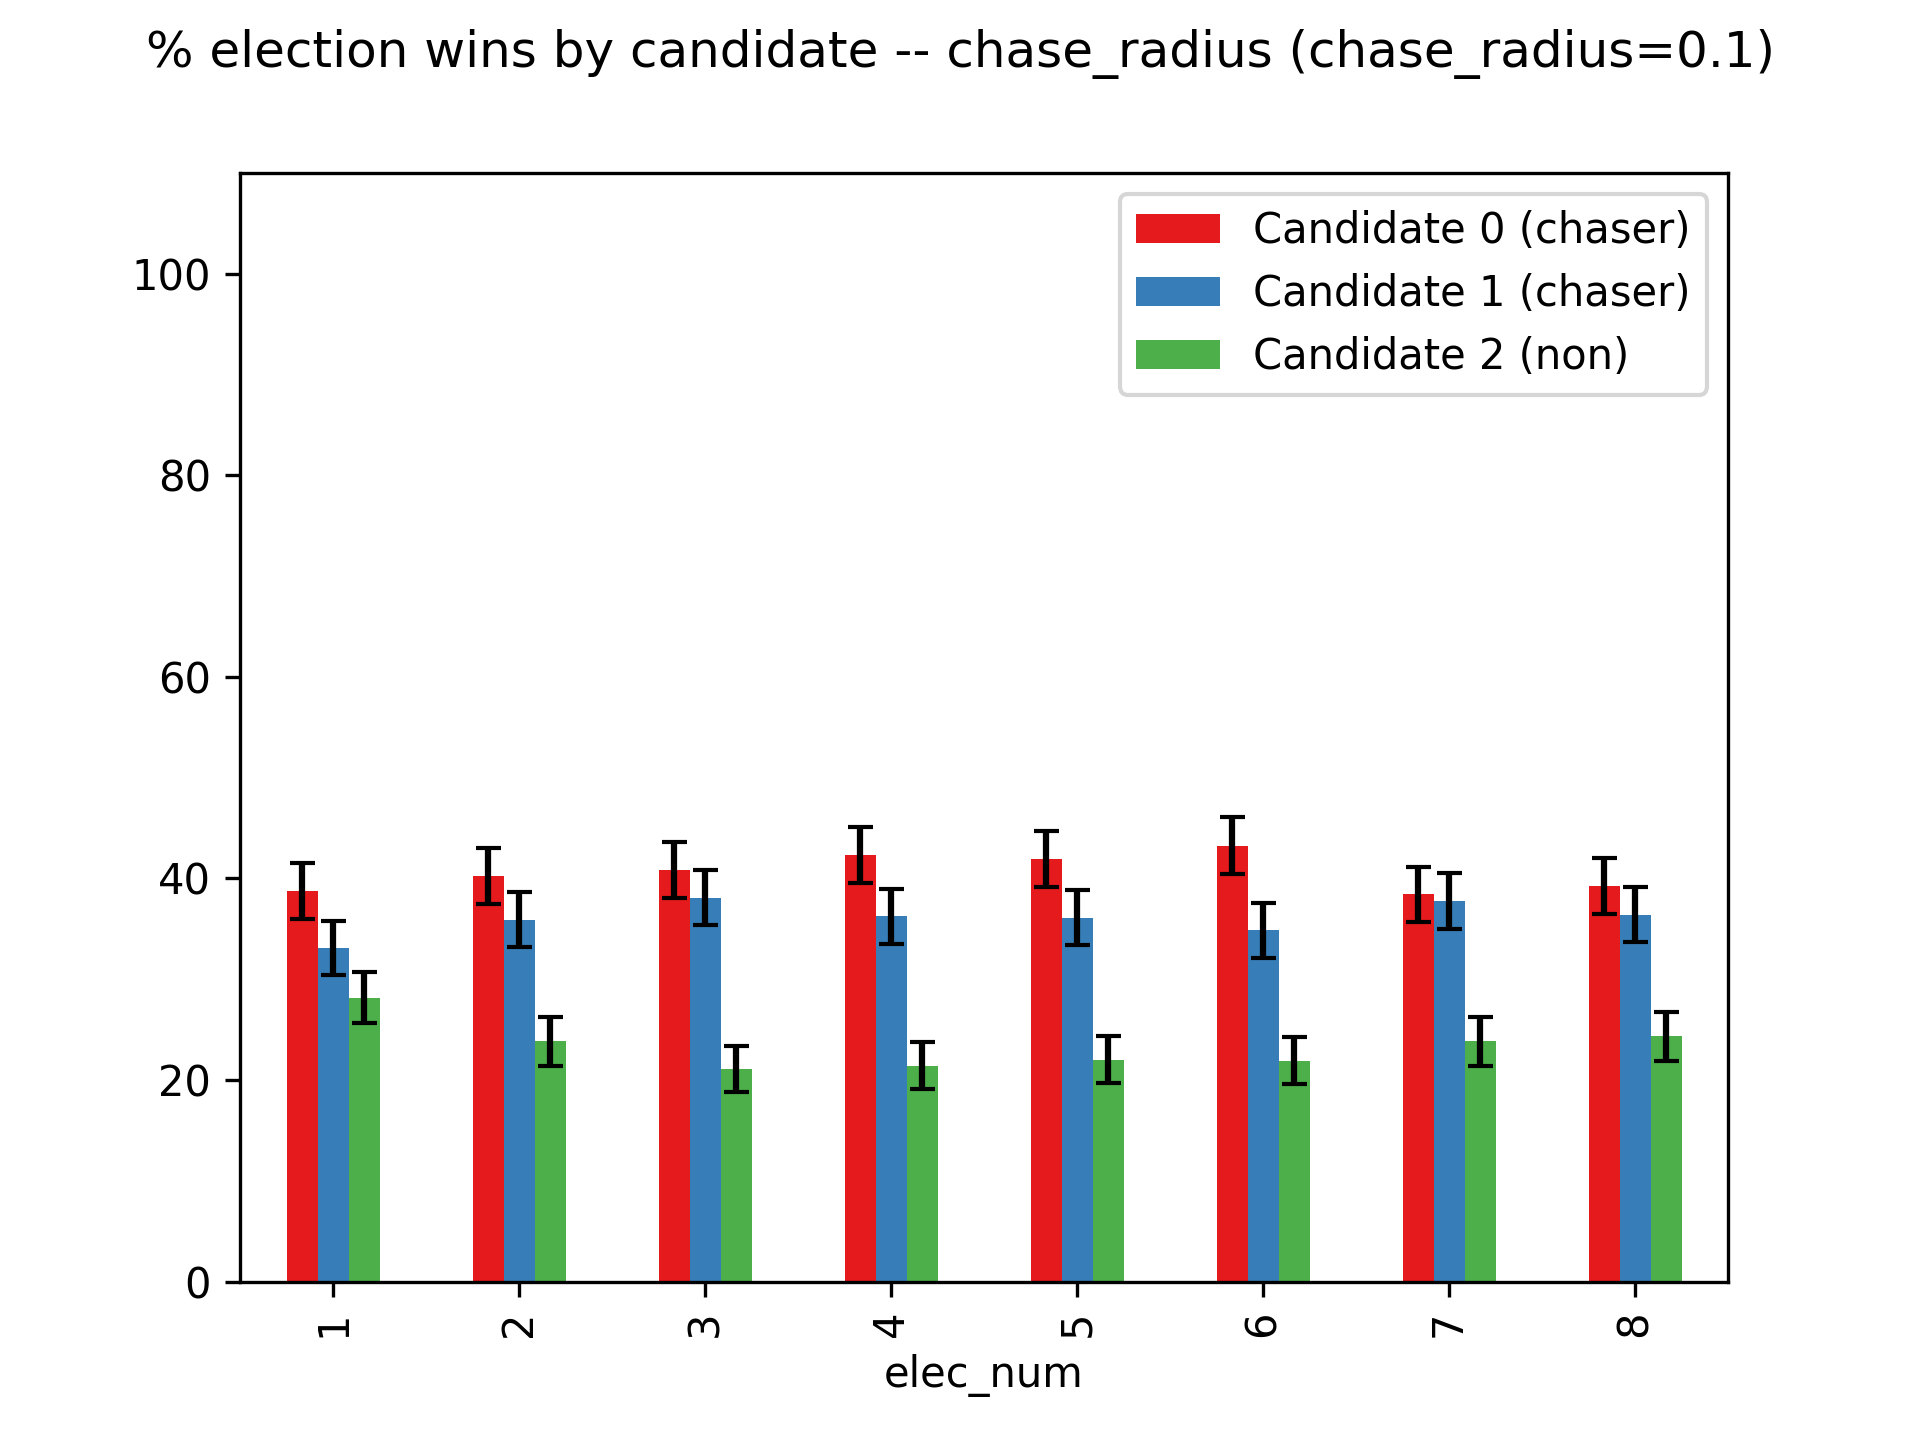
\includegraphics[width=0.31\textwidth]{assets/chase_radius_.1_winners.png}
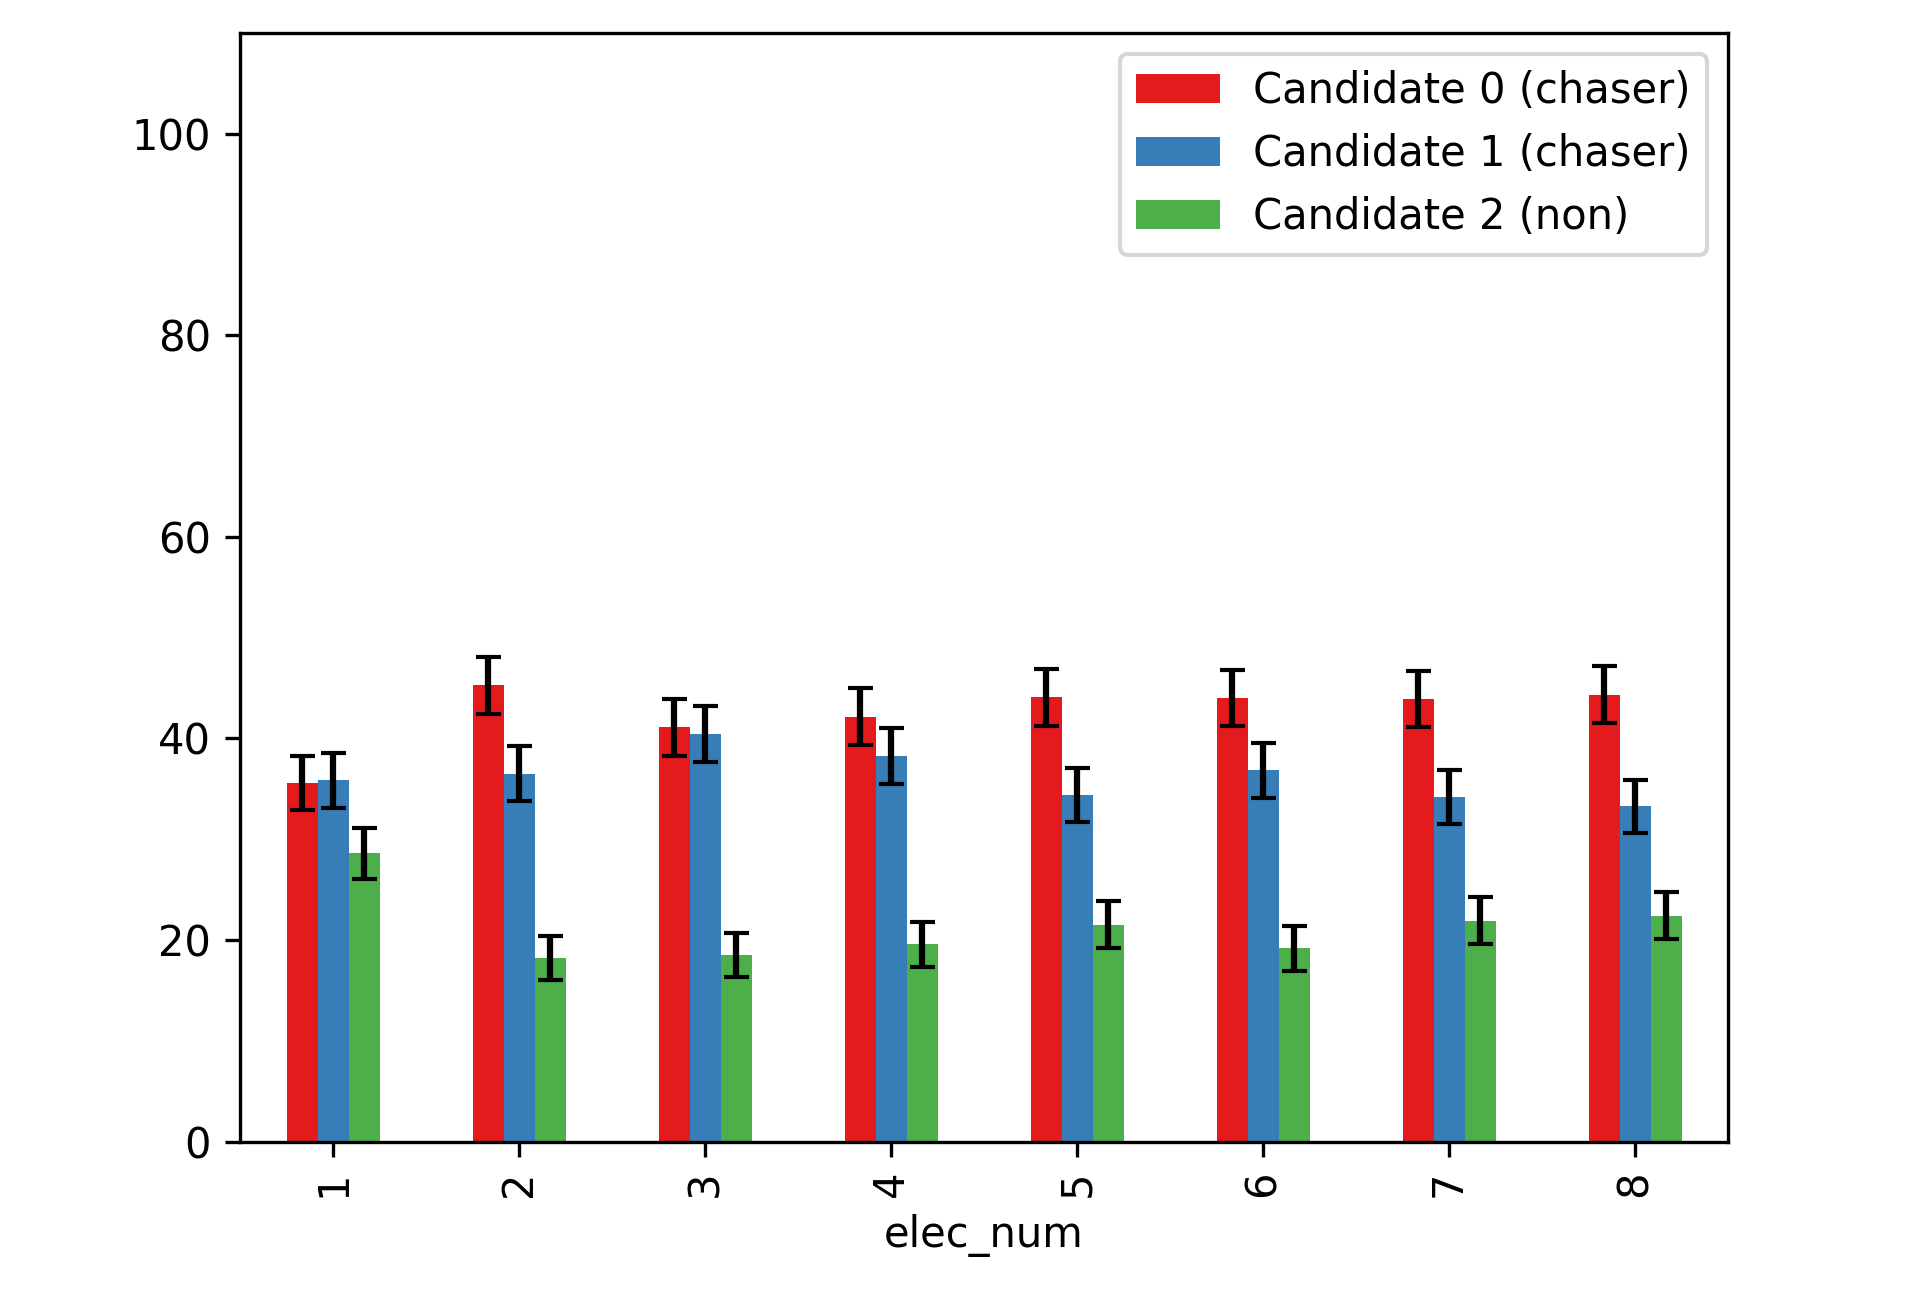
\includegraphics[width=0.31\textwidth]{assets/chase_radius_.2_winners.png}
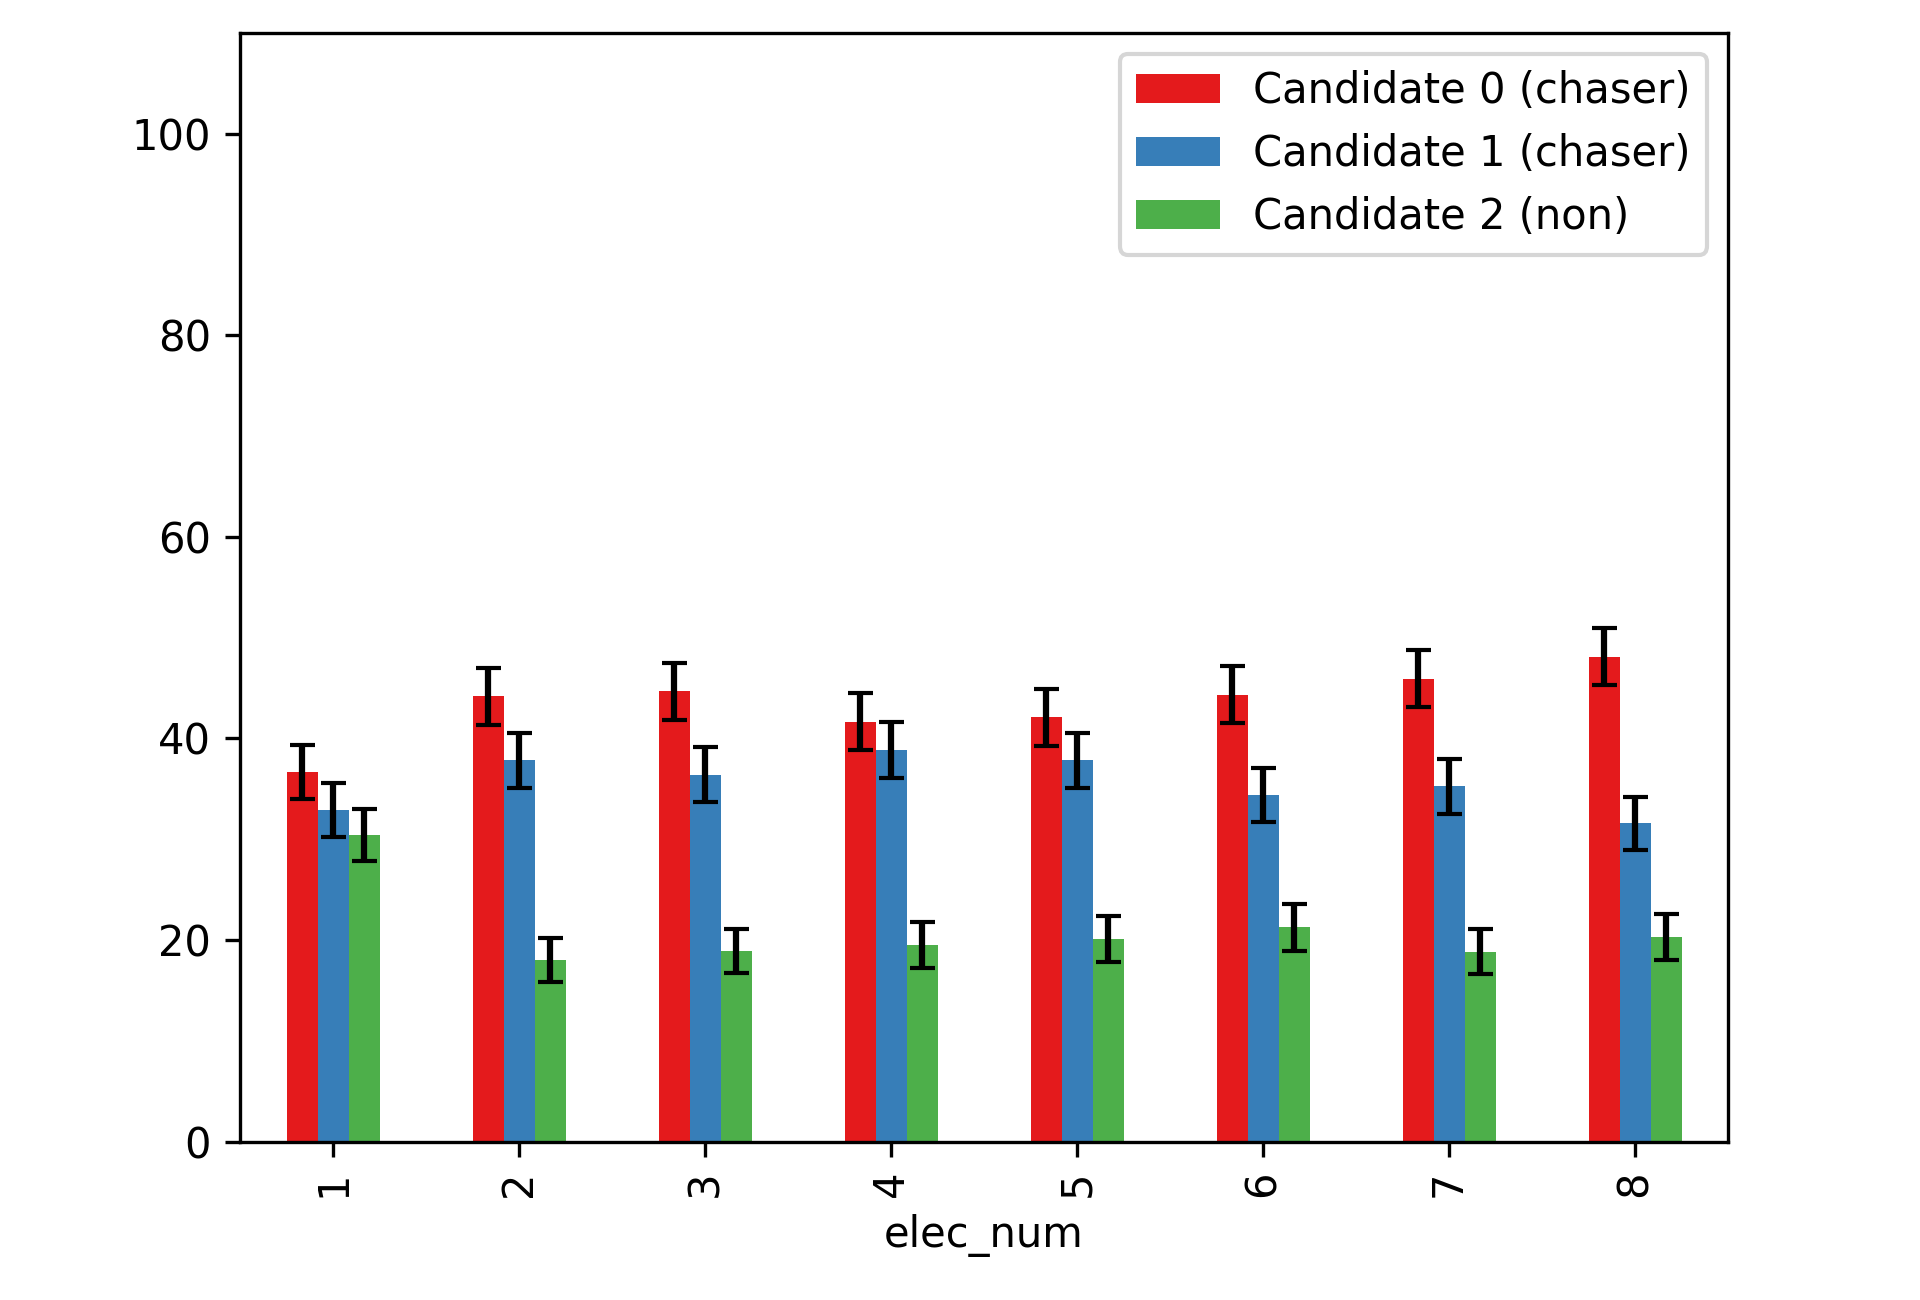
\includegraphics[width=0.31\textwidth]{assets/chase_radius_.3_winners.png}
\caption{Election winners when two chasers' chase radii are varied from .1 to
.2 to .3. The outcomes show negligible difference.}
\label{chase_radius}
\end{figure}

More interesting is when we make one chaser more aggressive than the other
(\textit{i.e.} more willing to take risky positions, and perhaps to abandon
their base and traditional platform). Figure~\ref{diff_chase_radius} shows the
chase distances and election win totals for two chasing candidates with
different chase radii: candidate 0's (red) is .1, and candidate 1's (blue) is
.2. As can be seen, at first candidate 1 makes much larger leaps in opinion
space in an effort to appeal to voters, but after six or seven election cycles
approaches candidate 0's distances. In the right half of the figure, we see
that the more aggressively-chasing candidate now ekes out election victories
its rival in all elections but the first, even with candidate 0 being awarded
ties.

\begin{figure}
\centering
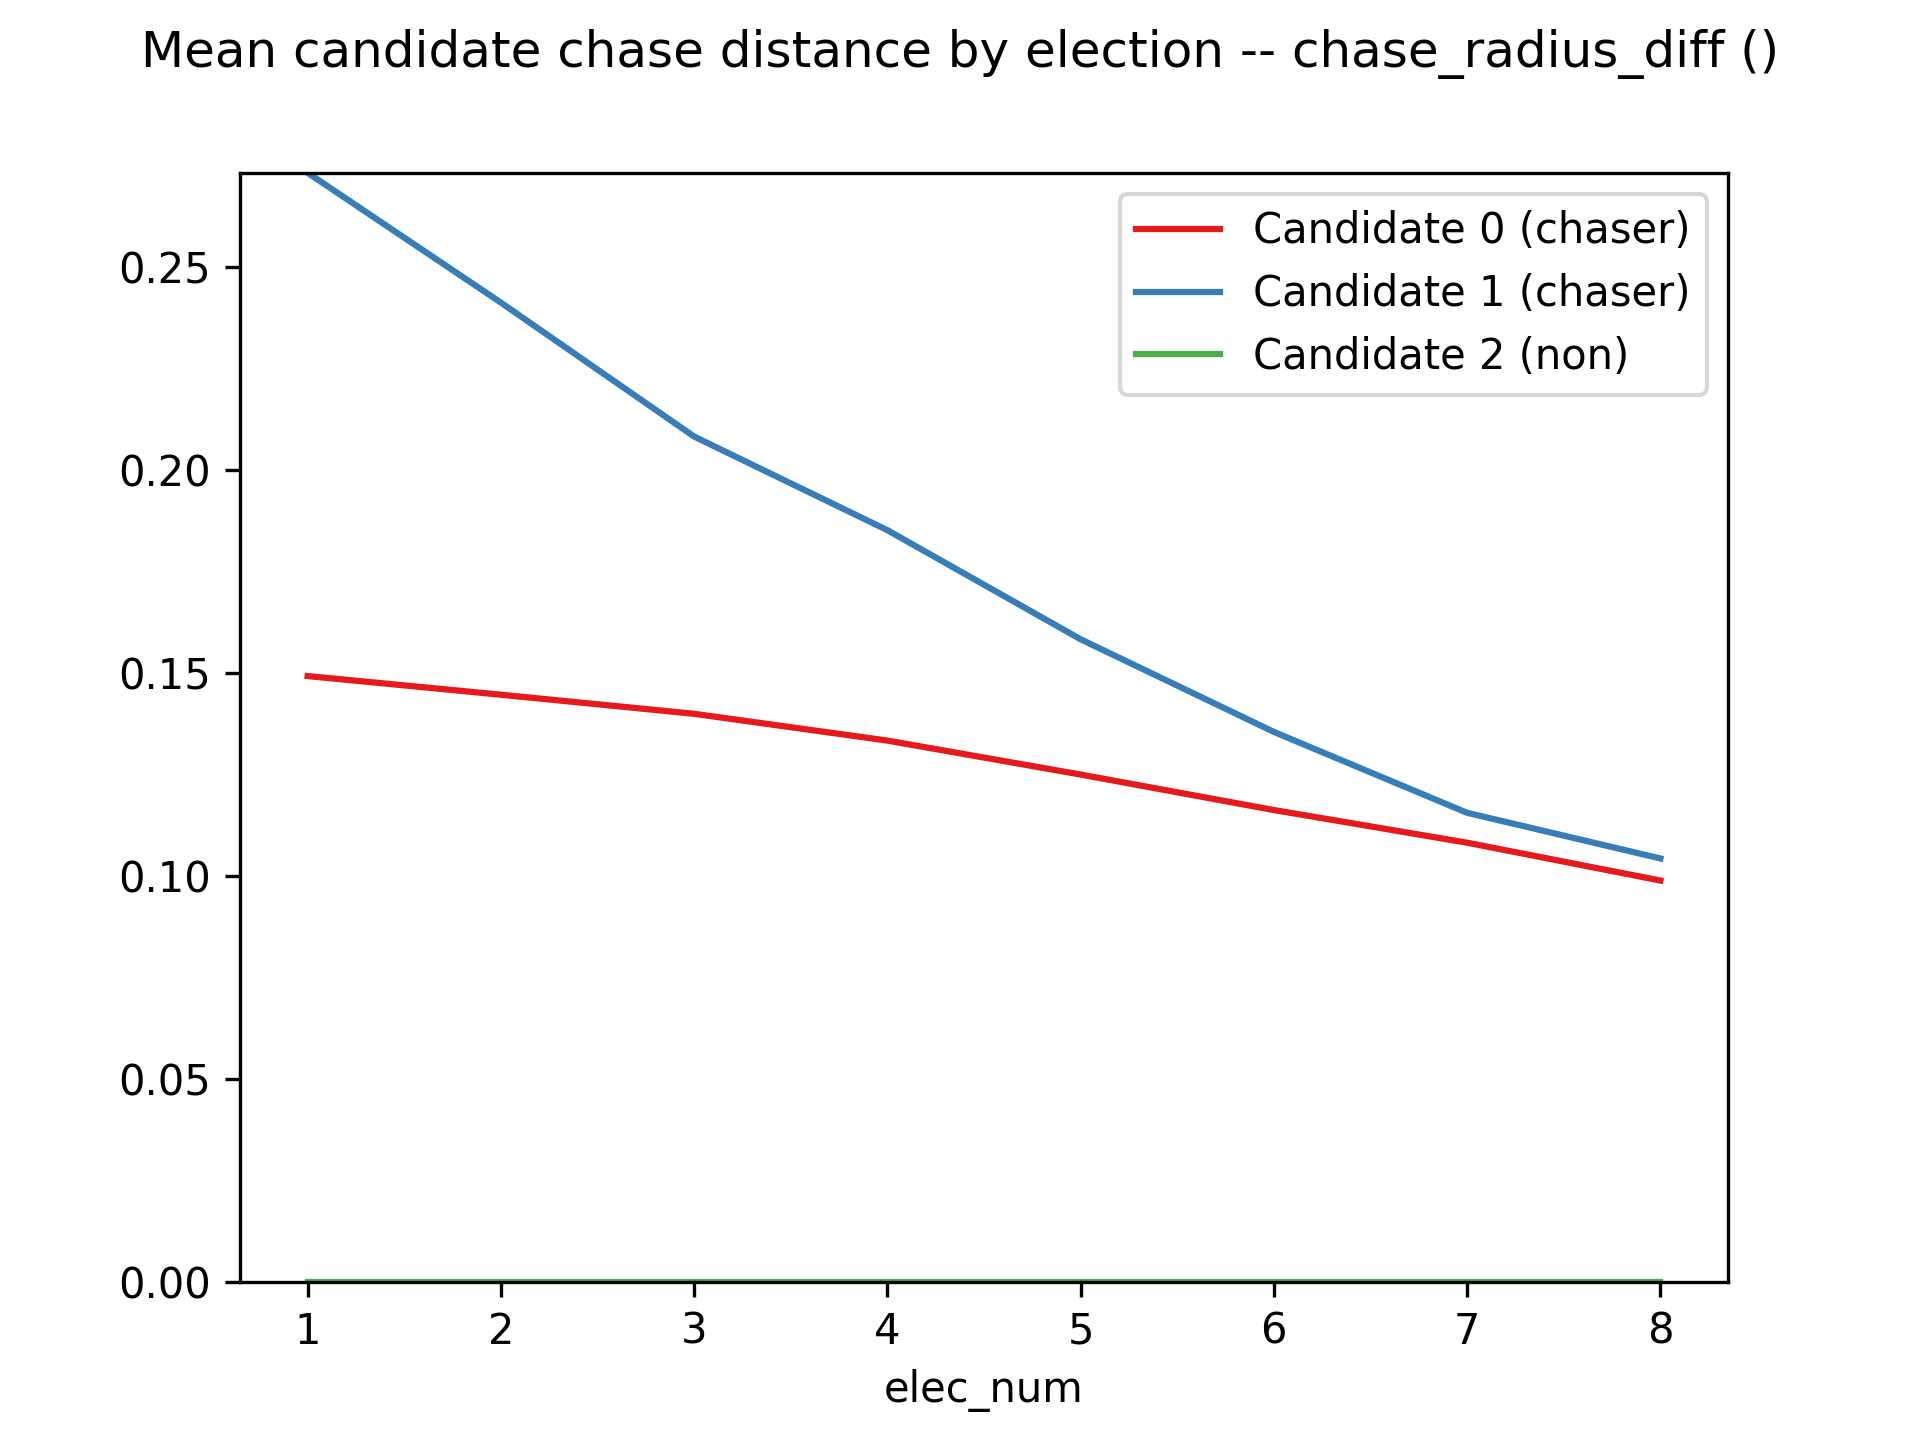
\includegraphics[width=0.45\textwidth]{assets/diff_chase_radii_dists.png}
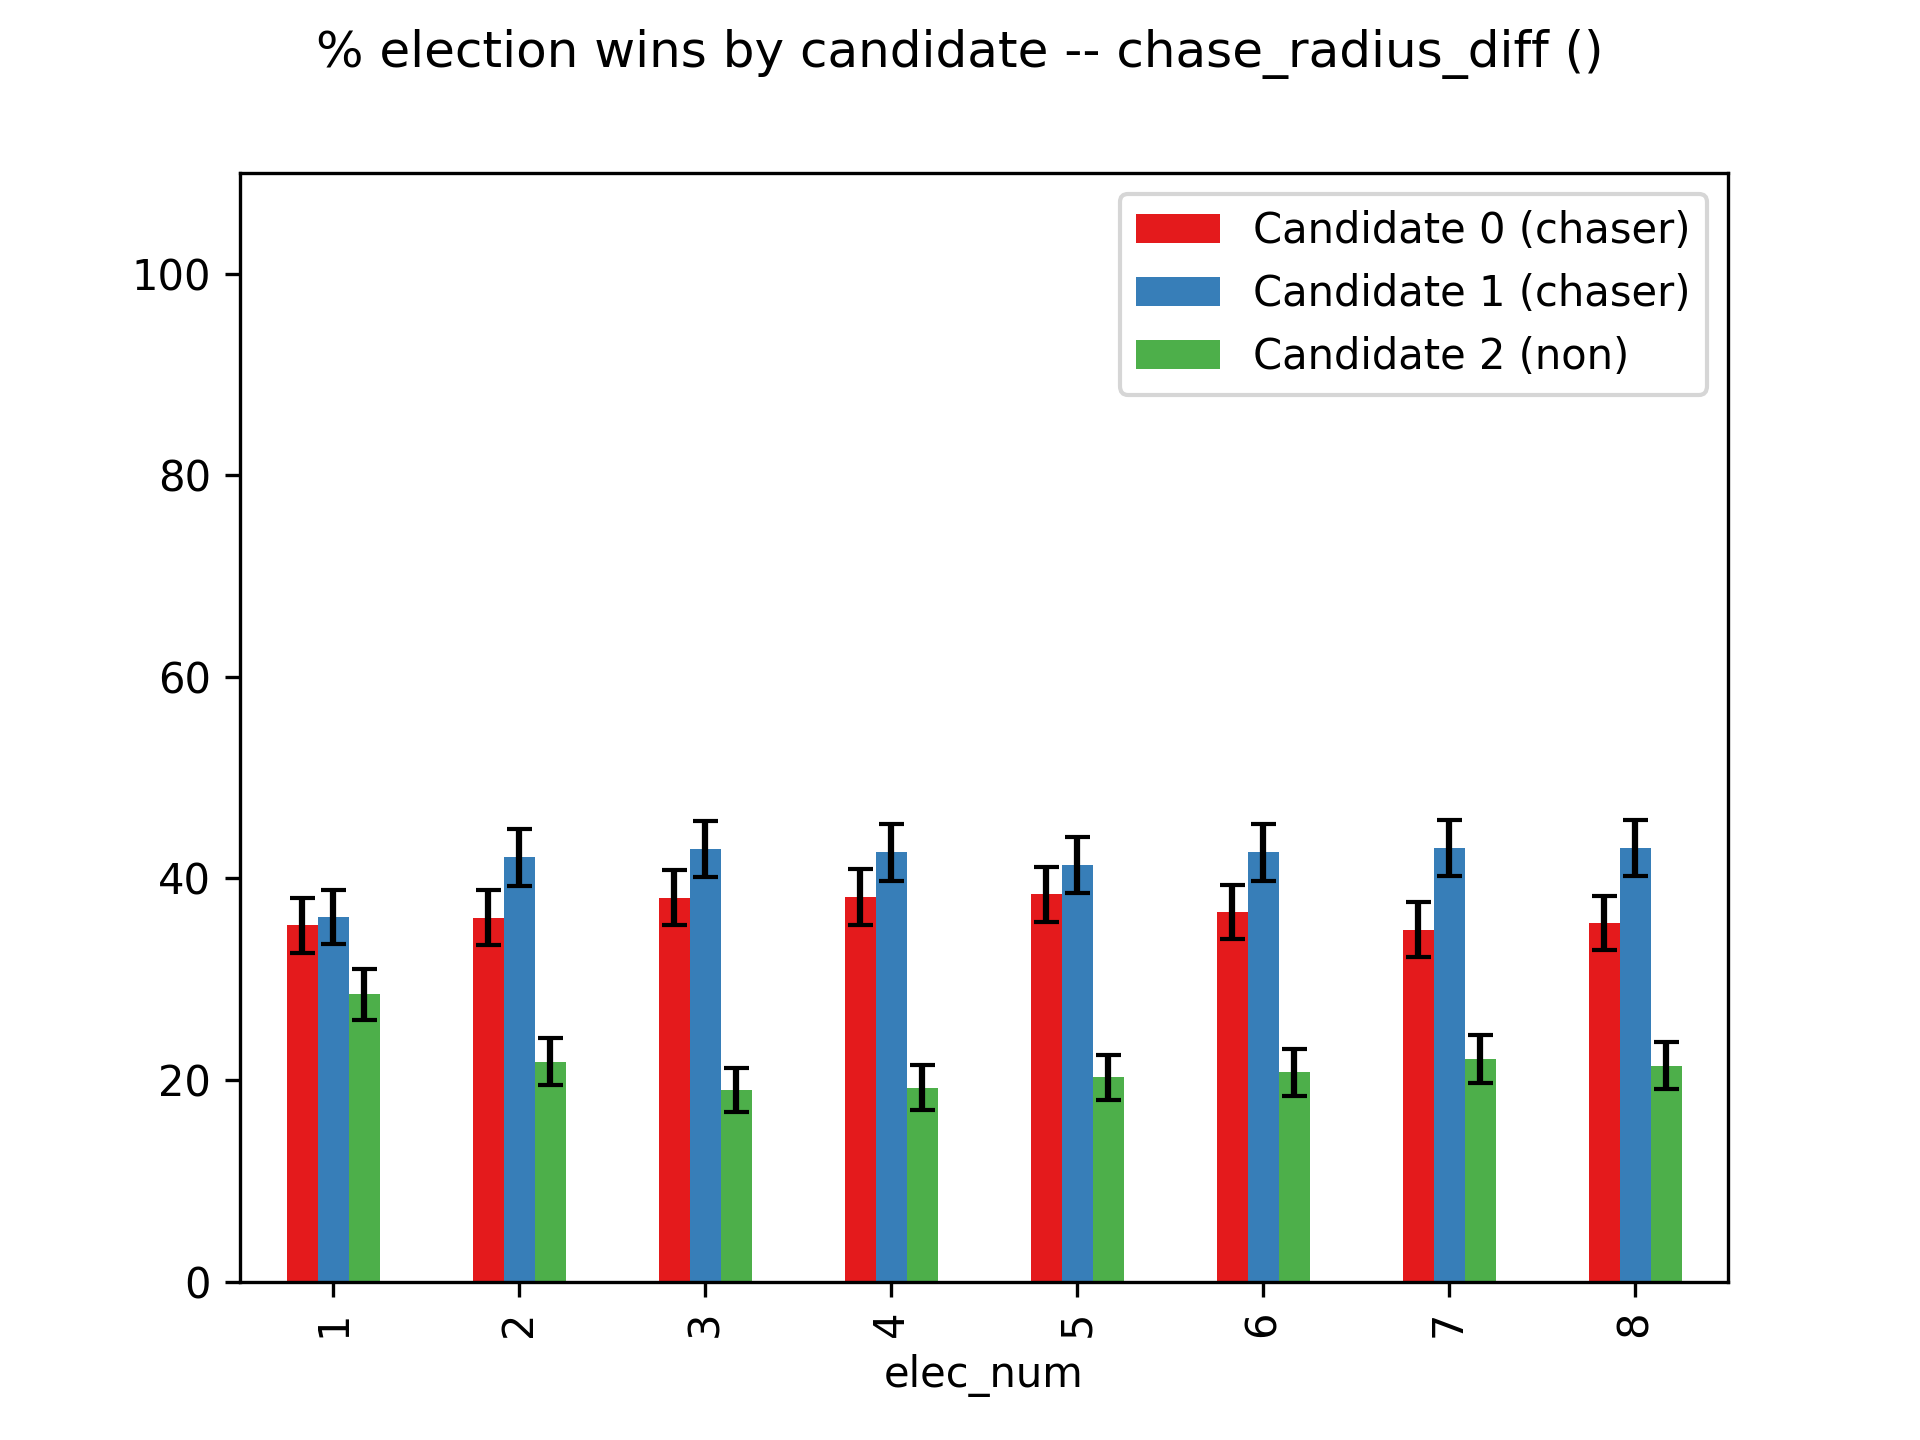
\includegraphics[width=0.45\textwidth]{assets/diff_chase_radii_winners.png}
\caption{Total chase distances, and election outcomes, for two chasing
candidates with different chase radii (candidate 0: radius 0.1; candidate 1:
radius 0.2) plus a non-chasing candidate.}
\label{diff_chase_radius}

\end{figure}

% Question for us to figure out: why, if default voter alg, only one chaser
% gets any benefit (two chasers cancel each others' benefits out stat sig) but
% if all voters are rational, then two chasers both benefit.


% Some preliminary findings and questions:

% chasing does pay off if lots of rational voters.
% chasing does not pay off if lots of party voters.
% Is there a correlation between how much each candidate chased (total sum of Euclidean distances of all chase actions) and how often they won

% does chasing ever hurt a candidate? hypothesis: if voters easily switch
% parties, and a candidate "overchases" and outruns their base, they will lose
% their base and this will hurt them. Can we reproduce this?

% Is there a correlation between how much the voting population is drifting and how likely the election at that time is to be rational?





\section{Discussion}
\label{sec:discussion}

\subsection{Candidate chasing}

%1. General findings about candidate "chasing." Do candidates tend to chase the
%same amount? Do high-chasers tend to do better in elections than low-chasers?
%Etc. **(SD)**

\subsection{Electorate's voting algorithm composition}

%2. General findings about voter algorithm mix. How much does this matter? How
%often are elections rational based on various compositions? Do certain voter
%algorithms make drifting less/more effective? **(HP)**

\section{Future work}
\label{sec:future}

% HP: pick 2 or three and discuss briefly

%More than, and less than, 3 candidates

%candidates chasing more often than just once per election (based on polling
%data between elections) ***

%the "constrained rational" voting alg

%different social network types and parameters ***

%issue importance (related to F\&F) ***

%a non-fixed voting population (voters enter/exit, influenced by parents)

One future point of exploration is testing the sensitivity of the model to network
variance. We used an  Erd\H{o}s-R\'{e}nyi graph,
but would like to test our model with different networks and edge probabilities.

Our next major step is to fit the model to empirical data by calibrating the
initial conditions and validating the outcomes with polling data. This would allow
us to model the effectiveness of vote-seeking campaigns in a real democratic
system, and arguably more importantly, identify feasible strategies to increase the 
rationality of elections.


\section{Conclusions and future work}
\label{sec:conclusions}



\bibliographystyle{scsproc}

\bibliography{assets/bib}



\section*{Author Biographies}

\textit{(To be redacted for initial blind submission.)}

\sout{\textbf{\uppercase{Stephen Davies}} is an international spy, sought-after
public speaker, and former member of the Jedi Council on Coruscant. He's
considered armed and dangerous and should be approached with caution.
His email address is \email{stephen@umw.edu}.}

\sout{\textbf{\uppercase{Harmony Peura}} is an Honors student in the University of
Mary Washington Computer Science department, and also sings alto for several
acapella groups. She has climbed Mt.~Everest on three separate occasions. Her
email address is \email{hpeura@umw.edu}.}


\end{document}
